\documentclass[11pt]{report}

% === Tiếng Việt
\usepackage[utf8]{vietnam}
\usepackage[vietnamese]{babel}
\usepackage{blindtext}

% ===== Thông tin
\newcommand{\at}{Đà Nẵng, ngày ..... tháng ..... năm 2022}
\newcommand{\project}{Hệ thống tạo và liên kết Sàn thương mại điện tử cho Nhà sản xuất và Cửa hàng}
\newcommand{\me}{Trần Ngọc Huy}
\newcommand{\advisor}{TS. Lê Thị Mỹ Hạnh}
\newcommand{\msv}{102180208}
\newcommand{\myclass}{18TCLC\_DT3}

% bảng có sang trang
\usepackage{longtable}


% ===== Căn chỉnh lề
\usepackage[
% >>> Page layout: cỡ giấy A4; lề trái: 3cm, lề phải: 2cm, lề trên: 2,5cm, lề dưới: 2,5cm;
a4paper,
left=3cm,
right=2cm,
top=2.5cm,
bottom=2.5cm,
% >>> header và footer: from edge: 1,6cm;
headsep=0.45cm
]{geometry}

% ==== Tiêu đề, chân trang
\usepackage{fancyhdr}




%	Chú dẫn bảng: nằm trên bảng, đánh số theo chương và số lũy tiến theo số thứ tự của
%	bảng trong chương;
%	Chú dẫn hình: nằm dưới hình, đánh số theo chương và số lũy tiến theo số thứ tự của
%	hình trong chương;
%	Đánh số công thức: bên phải công thức, đánh số theo chương và số lũy tiến theo số
%	thứ tự của công thức trong chương;
%	Nên sử dụng các chức năng về Bookmark, Caption, Cross-Reference, Format
%	Heading,... của Microsoft Word hoặc các phần mềm soạn thảo tương tự; cần tổ chức
%	theo dạng “Long Document”.



% ===== font Times
\usepackage{mathptmx}



% ==== Căn trái phải chữ
\usepackage[document]{ragged2e}


% ===== Khai báo hình ảnh
\usepackage{graphicx}
\graphicspath{ {images/} }
\renewcommand{\listtablename}{Danh sách các bảng, hình vẽ}

% ===== Bảng
\usepackage{multirow}


% ===== Danh mục từ viết tắt
\usepackage[toc]{glossaries}

\makeglossaries
\newacronym{mvc}{MVC}{Model View Controller}
\newacronym{sql}{SQL}{Structured Query Language}
\newacronym{no-sql}{No-SQL}{No Structured Query Language}
\newacronym{http}{HTTP}{Hypertext Transfer Protocol}
\newacronym{vps}{VPS}{Virtual Private Server}
\newacronym{html}{HTML}{HyperText Markup Language}
\newacronym{c}{C}{C programming language}
\newacronym{dbms}{DBMS}{cơ sở dữ liệu management system}
\newacronym{api}{API}{Application Programming Interface}
\newacronym{cod}{COD}{Cash On Delivery.}
\newacronym{url}{URL}{Uniform Resource Locator}
\newacronym{rest}{REST}{Representational state transfer}
\newacronym{ssl}{SSL}{Transport Layer Security}
\newacronym{csr}{CSR}{Client Side Render}
\newacronym{graphql}{GraphQL}{Graph Query Language}
\newacronym{json}{JSON}{JavaScript Object Notation}
\newacronym{bson}{BSON}{Binary Javascript Object Notation}
\newglossaryentry{dropshipping}
{
	name=dropshipping,
	description={phương pháp thực hiện bán lẻ mà một cửa hàng không lưu giữ sản phẩm được bán trong kho của mình.
	}
}

\newglossaryentry{request}{
	name=request,
	description={
		Là truy vấn theo giao thức HTTP.
	}
}

\newglossaryentry{headers}{
	name=Headers,
	description={
		Là một thành phần cấu trúc của truy vấn theo giao thức HTTP.
	}
}

\newglossaryentry{controller}{
	name=Controller,
	description={
		Bộ định tuyến truy cập trong mô hình MVC
	}
}

\newglossaryentry{id}{
	name=ID,
	description={
		Mã định danh
	}
}

\newglossaryentry{indexed}{
	name=indexed,
	description={
		Trong cơ sở dữ liệu indexed là kỹ thuật đánh dấu trường dữ liệu ưu tiên để sắp xếp và tìm kiếm.
	}
}


\newglossaryentry{mobile}{
	name=mobile,
	description={
		Thiết bị di động
	}
}


\newglossaryentry{backlog}{
	name=backlog,
	description={
		Sprint Backlog là bảng công việc được Nhóm Phát triển sử dụng để quản lý quá trình phát triển trong một Sprint
	}
}

\newglossaryentry{production}{
	name=production,
	description={
		Môi trường triển khai thực tế của một dự án.
	}
}

\newglossaryentry{staging}{
	name=staging,
	description={
		Môi trường triển khai thử nghiệm của một dự án.
	}
}
% ==== Chia cột
\usepackage{multicol}

% ==== Liên kết chỉ mục đến phần nội dung của nó.
\usepackage{hyperref}

% ==== Chèn code
\usepackage{listings}
\usepackage{xcolor}
\definecolor{codegreen}{rgb}{0,0.6,0}
\definecolor{codegray}{rgb}{0.5,0.5,0.5}
\definecolor{codepurple}{rgb}{0.58,0,0.82}
\definecolor{backcolour}{rgb}{0.95,0.95,0.92}
\lstdefinestyle{mystyle}{
	backgroundcolor=\color{backcolour},  
	commentstyle=\color{codegreen},
	keywordstyle=\color{magenta},
	numberstyle=\tiny\color{codegray},
	breakatwhitespace=false,     
	breaklines=true,         
	captionpos=b,          
	keepspaces=true,         
	numbers=left,          
	numbersep=5pt,         
	showspaces=false,        
	showstringspaces=false,
	showtabs=false,         
	tabsize=2,
	xleftmargin=10pt,
	xrightmargin=10pt,
}

\lstset{
	style=mystyle,
}

% ===== Gỡ bỏ nhảy trang sau mỗi section

\newcommand{\sectionbreak}{\clearpage}

% ==== Tùy chỉnh tiêu đề
% >>> {font: TimeNew Roman, bolt, size: 14, căn lề: center}
\usepackage{titlesec}


\titleformat{name=\chapter} % command
[hang] % shape
{
	\fontsize{14px}{14px}\centering\bfseries
} % format
{\centering{CHƯƠNG ~\thechapter}} % label
{14px} % sep
{}

\titlespacing*{\chapter}{0pt}{-14px}{14px}

\titleformat{name=\chapter, numberless} % command
[hang] % shape
{
	\fontsize{14px}{14px}\centering\bfseries
} % format
{\centering} % label
{14px} % sep
{}

\titlespacing*{\chapter}{0pt}{-14px}{28px}

\titleformat{\section}
{\normalfont\fontsize{13px}{13px}\bfseries}{\thesection}{1em}{}

\titleformat{\subsection}
{\normalfont\fontsize{13px}{13px}\bfseries\slshape}{\thesubsection}{1em}{}

\titleformat{\subsubsection}
{\normalfont\fontsize{13px}{13px}}{\bfseries\thesubsection}{1em}{}



% ==== Tạo ô tích
\usepackage{amssymb}


% khoảng cách dòng 
\linespread{1.45} 

\usepackage[above]{placeins}

% ==== Bảng nâng cao
\usepackage{tabularx}

% ==== Chỉnh font chữ cho list
\usepackage{enumitem}

%%%%%%%%%%%%%%%%%%%%%%%%%%%%%%%%%%%%%%%%%%%%%%%%%

\begin{document}

	\pagenumbering{gobble}
	% Trang trắng này dùng để dán bản Nhận xét của người hướng dẫn, hoặc thay trang này bằng Nhận xét của người hướng dẫn
	\chapter*{NHẬN XÉT CỦA NGƯỜI HƯỚNG DẪN}
	\dotfill\\\dotfill\\\dotfill\\\dotfill\\\dotfill
	\\\dotfill\\\dotfill\\\dotfill\\\dotfill\\\dotfill
	\\\dotfill\\\dotfill\\\dotfill\\\dotfill\\\dotfill
	\\\dotfill\\\dotfill\\\dotfill\\\dotfill\\\dotfill
	\\\dotfill\\\dotfill\\\dotfill\\\dotfill\\\dotfill
	\\\dotfill\\\dotfill\\\dotfill\\\dotfill\\\dotfill
	\\\dotfill\\\dotfill\\\dotfill\\
	\pagebreak
	
	% Trang trắng này dùng để dán bản Nhận xét của người phản biện, hoặc thay trang này bằng Nhận xét của người phản biện
	\chapter*{NHẬN XÉT CỦA NGƯỜI PHẢN BIỆN}
	\dotfill\\\dotfill\\\dotfill\\\dotfill\\\dotfill
	\\\dotfill\\\dotfill\\\dotfill\\\dotfill\\\dotfill
	\\\dotfill\\\dotfill\\\dotfill\\\dotfill\\\dotfill
	\\\dotfill\\\dotfill\\\dotfill\\\dotfill\\\dotfill
	\\\dotfill\\\dotfill\\\dotfill\\\dotfill\\\dotfill
	\\\dotfill\\\dotfill\\\dotfill\\\dotfill\\\dotfill
	\\\dotfill\\\dotfill\\\dotfill\\
	\pagebreak

	\fontsize{13px}{13px}\selectfont\justifying

\clearpage
\addcontentsline{toc}{chapter}{TÓM TẮT}
\chapter*{TÓM TẮT}
\fontsize{13px}{13px}\selectfont\justifying

\raggedright
Tên đề tài: \project\\
Sinh viên thực hiện: ...\me \dotfill\\
Số thẻ sinh viên: ........ \msv \dotfill\\
Lớp sinh hoạt: ............ \myclass \dotfill\\
% >>> {Nội dung tóm tắt trình bày tối đa trong 1 trang} {Font: Time New Roman; thường; cỡ chữ: 13; dãn dòng: 1,3; căn lề: justified}
\vspace{14px}
\justifying
Trong thời kỳ cả nước thúc đẩy khởi nghiệp \cite{ocop}. Các mô hình, sản phẩm nông nghiệp, thủ công, truyền thống liên tục ra đời và cải tiến nâng cao chất lượng và quy mô sản xuất. Quá trình trên giúp cho sản phẩm ngày một đa dạng. Tính truyền thống, đặc trưng vùng miền có cơ hội phát triển.

Đồ án phát triển giải pháp giúp cho những đơn vị chủ thể tạo kênh thông tin với chi phí thấp. Các cửa hàng phân phối những sản phẩm trên có sàn thương mại riêng để chủ động truyền thông theo cách riêng. Việc xây dựng hệ thống trên, đồng thời cũng phát triển được sự liên kết thông tin giữa các đơn vị với nhau. Tránh sự lãng phí về nhân lực trong quá trình đồng bộ dữ liệu.

% Định hướng tạo nên đột phá cho đồ án sẽ được phát triển khi dữ liệu khách hàng và số lượng các nhà sản xuất đủ lớn. Khi đó vấn đề gần nhất cần giải quyết là hệ thống gợi ý giá bán và thu thập thông tin phản hồi từ khách hàng để cải thiện quá trình sản xuất.
	
\pagebreak

	\fontsize{13px}{13px}\selectfont\justifying

\addcontentsline{toc}{chapter}{NHIỆM VỤ ĐỒ ÁN }
	% ĐƠN VỊ
	\begin{minipage}[t]{.5\textwidth}
		\centering
		ĐẠI HỌC ĐÀ NẴNG\\
		\textbf{TRƯỜNG ĐẠI HỌC BÁCH KHOA}\\
		\underline{KHOA CÔNG NGHỆ THÔNG TIN}
	\end{minipage}\hfill 
	% QUỐC HIỆU TIÊU NGỮ
	\begin{minipage}[t]{.5\textwidth}
		\centering
		\textbf{CỘNG HÒA XÃ HỘI CHỦ NGHĨA VIỆT NAM}\\
		\underline{Độc lập - Tự do - Hạnh phúc}
	\end{minipage}\\[2em]
	
	\center\Large\textbf{NHIỆM VỤ ĐỒ ÁN TỐT NGHIỆP}
	\vspace{14px}
	\fontsize{12px}{12px}\selectfont
	
	Sinh viên thực hiện: \emph\me \dotfill Số thẻ sinh viên: \emph\msv \dotfill 
	
	Lớp: \emph\myclass \dotfill Khoa: \emph{Công nghệ thông tin} \dotfill Ngành: \emph{Công nghệ Phần Mềm} \dotfill
	
	\begin{enumerate}[before=\fontsize{13px}{13px}\selectfont]
		\item\emph{Tên đề tài đồ án: \project\dotfill}
		\item\emph{Đề tài thuộc diện: $\square$ Có ký kết thỏa thuận sở hữu trí tuệ đối với kết quả thực hiện}
		\item\emph{Các số liệu và dữ liệu ban đầu: Không\dotfill}
		\item\emph{Nội dung các phần thuyết minh và tính toán:}
		Phần mở đầu mô tả chung về đồ án. Nêu vấn đề và phương pháp giải quyết.
		\begin{itemize}
			\item \textbf{Chương cơ sở lý thuyết} nêu ra các nền tảng, công nghệ, công cụ, dịch vụ làm cơ sở để phát triển đồ án.
			\item \textbf{Chương phân tích thiết kế} nêu ra các yêu cầu đặc tả, trình bày sơ đồ hành vi, sơ đồ cấu trúc của đồ án.
			\item \textbf{Chương triển khai và đánh giá} trình bày kết quả đạt được, các hoạt động đã triển khai và đánh giá mức độ hoàn thiện so với yêu cầu đề ra.
		\end{itemize}
		\item\emph{Các bản vẽ, đồ thị ( ghi rõ các loại và kích thước bản vẽ ):}
		\begin{itemize}
			\item Sơ đồ ca sử dụng
			\item Sơ đồ hoạt động
			\item Sơ đồ lớp
			\item Sơ đồ khối thành phần
			\item Sơ đồ triển khai
		\end{itemize}
		\item\emph{Họ tên người hướng dẫn: \advisor}
		\item\emph{Ngày giao nhiệm vụ đồ án: ...../...../ 2022 \dotfill}
		\item\emph{Ngày hoàn thành đồ án: ...../...../ 2022 \dotfill}
		
	\end{enumerate}
	\raggedright
	% ĐƠN VỊ
	\begin{minipage}[t]{.5\textwidth}
		
		\textbf{Trưởng bộ môn} \dotfill
	\end{minipage}\hfill 
	\begin{minipage}[t]{.5\textwidth}
		\center
		\at\\
		\textbf{Người hướng dẫn}
	\end{minipage}\\[2em]
	\pagebreak
	
	% Đánh số trang la mã
	\pagenumbering{roman}
	\setcounter{page}{1}
	% Lời nói đầu

	\fontsize{13px}{13px}\selectfont\justifying

\clearpage
\addcontentsline{toc}{chapter}{LỜI NÓI ĐẦU}
\chapter*{LỜI NÓI ĐẦU}
	\fontsize{13px}{13px}\selectfont\justifying
	Ngành công nghệ phần mềm nghiên cứu về các kỹ thuật, phương pháp, hạ tầng của phần mềm máy tính. Người phát triển phần mềm không đơn giản là chỉ cần biết đến ngôn ngữ lập trình là có thể phát triển được hết. Sau thời gian học tập và nghiên cứu tại trường Đại Học Bách Khoa Đà Nẵng. Cùng với sự thực hành miệt mài và những kinh nghiệm, tư duy, định hướng ngoài giờ lên lớp từ các thầy cô. Em nhận thấy bản thân tiến bộ toàn diện, không chỉ các kiến thức chuyên ngành. Các phương pháp nghiên cứu, tinh thần học tập, tư duy giải quyết vấn đề,... cũng ngày một hoàn thiện.
	% Các bạn tân sinh viên có thể thắc mắc rằng vai trò của trường Đại học là gì trong thời kì kiến thức mở. Nếu các bạn thấy được mục tiêu và định hướng của mỗi người là khác nhau khi họ tiếp xúc với những cộng đồng khác nhau. Thì các bạn sẽ nhận ra rằng: bạn bè, thầy cô, giáo trình, cơ sở vật chất tốt không cải thiện năng lực của bạn. Đó là môi trường phát triển. Đơn giản nếu xem năng lực của cá nhân là sản phẩm của tư duy, thì môi trường là \emph{"nguyên liệu"} của sản phẩm đó. Nó cần quá trình chế tác bởi chính năng lực tư duy của bạn. Hiểu được như vậy sẽ không còn nhập nhằng giữa các quan điểm \emph{"Giỏi thì ở đâu cũng giỏi"} hay \emph{"Không thầy đố mày làm nên"}.
	
	Đề tài này là kết quả của quá trình học tập tại trường Đại Học Bách Khoa Đà Nẵng. Không chỉ dừng lại ở mức độ là một luận án tốt nghiệp. Những hạn chế tồn đọng sẽ được tiếp tục hoàn thiện khi năng lực và điều kiện phát triển. Đồ án sẽ tiếp tục triển khai và hướng đến công năng thực tế cho các chủ thể hộ kinh doanh, doanh nghiệp. .
	
	Cuối cùng em xin cảm ơn thầy cô và bạn bè đã đồng hành cùng em trong suốt năm tháng vừa qua. Cảm ơn cô Lê Thị Mỹ Hạnh đã hướng dẫn em hoàn thành đồ án, luận văn tốt nghiệp. Em xin chân thành cảm ơn!	
	\pagebreak
	% Cam đoan
	\fontsize{13px}{13px}\selectfont\justifying

\addcontentsline{toc}{chapter}{CAM ĐOAN}
	\chapter*{CAM ĐOAN}
	% >>> {Font: Time New Roman; thường; cỡ chữ: 13; dãn dòng: 1,3; căn lề: justified} {Lời cam đoan của sinh viên thực hiện đồ án tốt nghiệp cam đoan về liêm chính học thuật}
	\fontsize{13px}{13px}\selectfont\justifying
	
	Tôi xin cam đoan:
	\begin{itemize}
		\item Báo cáo đồ án tốt nghiệp đề tài: \emph{\project} là công trình nghiên cứu của chính cá nhân tôi dưới sự hướng dẫn trực tiếp của giảng viên \advisor.
		\item Tôi đã tự đọc nghiên cứu, dịch tài liệu và tổng hợp các kiến thức đã làm nên báo cáo này và đảm bảo không sao chép ở bất cứ đâu.
		\item Những lý thuyết trong luận văn đều được sử dụng tài liệu như tôi đã tham khảo ở phần tài liệu tham khảo đã có trong báo cáo. Nếu có vi phạm, tôi xin chịu hoàn toàn trách nhiệm.
	\end{itemize}
	
	\vspace{1cm}
	
	\hspace*{\fill}
	\begin{tabular}{c} %% if you want centered alignment use 'c' instead of 'l'
		{\large Sinh viên thực hiện}
		\vspace{3cm}\\
		\me
	\end{tabular}
	
	
	


	


	% Mục lục
	%{Để 2 dòng trống tại đây} {Font: Time New Roman; thường; cỡ chữ: 13; dãn dòng: 1,3; căn lề: justified} {In trên 2 mặt giấy từ trang này đến hết phần “PHỤ LỤC”}\\

	\fontsize{13px}{13px}\selectfont\justifying
	\renewcommand*\contentsname{MỤC LỤC}
	\addcontentsline{toc}{chapter}{MỤC LỤC}
	\cleardoublepage
	\tableofcontents
	
	\renewcommand{\listfigurename}{DANH SÁCH HÌNH VẼ}
	\renewcommand{\listtablename}{DANH SÁCH BẢNG}
	\listoffigures
	\listoftables
	\addcontentsline{toc}{chapter}{DANH SÁCH BẢNG VÀ HÌNH VẼ}

	\printglossary[title={DANH SÁCH CÁC KÝ HIỆU, CHỮ VIẾT TẮT}, toctitle={DANH SÁCH CÁC KÝ HIỆU, CHỮ VIẾT TẮT}]
	
	% ===== Nội dung đồ án =====
	% >>> Mục Header: Tên đề tài (định dạng: font Time New Roman, Italic, size 10, căn lề: giữa);
	% header đầu chương
		\fancypagestyle{plain}{%
		\fancyhf{}%
		\fancyhead[CE,CO]{\fontsize{10px}{10px}\selectfont\emph{{\project}}}
	}
	% headers bình thường
	\pagestyle{fancy}
	\fancyhf{}
	\fancyhead[CE,CO]{\fontsize{10px}{10px}\selectfont\emph{{\project}}}
	
	% >>> Mục Footer: Sinh viên thực hiện, giảng viên hướng dẫn, đánh số trang (định dạng: font Time New Roman, size 10);
	\fancyfoot[LE,LO]{{\normalsize {Thực hiện: \me}}
	}
	\fancyfoot[CE,CO]{{\normalsize {Hướng dẫn: \advisor}}	
	}
	\fancyfoot[LE,RO]{\thepage}
	% đường kẻ
	\renewcommand{\headrulewidth}{0.3pt}
	\renewcommand{\footrulewidth}{0.3pt}
	\clearpage
	
	% Bắt đầu đánh số thứ tự arabic
	% Đánh số trang: bắt đầu đánh số trang từ phần “MỞ ĐẦU”;
	\pagenumbering{arabic}
	\setcounter{page}{1}
	%
	\fontsize{13px}{13px}\selectfont\justifying

\chapter*{MỞ ĐẦU}
\addcontentsline{toc}{part}{MỞ ĐẦU}
\subsection*{Vấn đề}

Tìm kiếm đầu ra cho sản phẩm là vấn đề hết sức quan trọng đối với đơn vị sản xuất. Một trong những kênh bán hàng hiệu quả có thể kể đến đó là chương trình triển lãm hội chợ, phân phối tại các cửa hàng.

Tuy nhiên, đối với các doanh nghiệp khởi nghiệp. Sản phẩm được cải tiến cập nhật thông tin liên tục. Sản lượng không đủ lớn để phân phối rộng. Web là một công cụ tuyệt vời để đăng tải các thông tin cần thiết thay vì in trực tiếp lên bao bì của sản phẩm. Nó cũng giúp doanh nghiệp quảng bá sản phẩm. Giúp khách hàng tìm kiếm tra cứu nhiều thông tin hơn.

\textbf{Về việc phát triển web.}\label{pro:1} Do nguồn lực không đủ, rất nhiều hộ kinh doanh, doanh nghiệp khởi nghiệp không thể xây dựng một Web với các thông tin cơ bản. Việc cập nhập thường xuyên thông tin sản phẩm cũng mất rất nhiều thời gian công sức của chủ thể.

\textbf{Về việc phân phối thông tin.}\label{pro:2} Khi thông tin sản phẩm được đăng tải  lên các trang thương mại điện tử khác hoặc trang web của các cửa hàng địa phương. Việc cập nhật và điều chỉnh giá là hết sức tốn thời gian.

Giải quyết các vấn đề nêu trên có thể xem như việc tạo tự động các sàn thương mại điện tử với hình thức \gls{dropshipping} cho nhà sản xuất hoặc xử lý đơn có lưu kho cho cửa hàng.

%\pagebreak
%
%\subsection*{Giải pháp}
%\addcontentsline{toc}{section}{Giải pháp}	

\subsection*{Giải pháp}

Đồ án cung cấp công cụ tạo trang thông tin sản phẩm riêng cho từng nhà sản xuất. Và cũng có thể chia sẻ dữ liệu sản phẩm cho các các cửa hàng. Các đơn vị phân phối và triển lãm có thể tích hợp trực tiếp dữ liệu gốc vào hệ thống của họ. Chủ động được phương pháp truyền thông mà không phụ thuộc vào sàn thương mại điện tử bên khác.

Đồ án xác định đối tượng trực tiếp phục vụ làm cơ sở để phát triển tính năng là khách mua hàng.

\begin{itemize}
	\item Khách hàng là người ủng hộ sử dụng nông sản chất lượng.
	\item Khách mua hàng tin tưởng chất lượng sản phẩm đăng tải trên trang.
	\item Khách hàng cảm thấy tiện lợi trong quy trình mua hàng.
	\item Khách hàng được tư vấn thông tin đầy đủ về giá trị sử dụng của sản phẩm.
	\item Khách hàng dễ dàng tìm kiếm sản phẩm phù hợp với nhu cầu.
\end{itemize}
Nhà bán hàng là người trả tiền cho hệ thống. Thông qua việc phục vụ người mua nông sản. Hệ thống gián tiếp đem lại giá
trị cho nhà bán hàng.
\begin{itemize}
	\item Không gian mở rộng.
	\item Thời gian linh hoạt.
	\item Khách hàng tiềm năng.
	\item Phù hợp với quy mô.
\end{itemize}

	
	\fontsize{13px}{13px}\selectfont\justifying

	\chapter{CƠ SỞ LÝ THUYẾT}

	\fontsize{13px}{13px}\selectfont\justifying
	% {font: TimeNew Roman, bolt, size: 14, căn lề: center}
	\section{Môi trường}
	
	\subsection{Trình duyệt}\label{subsection:webclient}
	Trình duyệt \cite{browser:what} web đưa bạn đến mọi nơi trên internet, cho phép bạn xem văn bản, hình ảnh và video từ mọi nơi trên thế giới.
	
	Web là một công cụ rộng lớn và mạnh mẽ. Trong một vài thập kỷ, Internet đã thay đổi cách chúng ta làm việc, cách chúng ta chơi và cách chúng ta tương tác với nhau. Tùy thuộc vào cách nó được sử dụng, nó là cầu nối giữa các quốc gia, thúc đẩy thương mại, nuôi dưỡng các mối quan hệ, thúc đẩy động cơ đổi mới của tương lai và chịu trách nhiệm về nhiều hơn những gì chúng ta biết phải làm.
	
	Điều quan trọng là mọi người đều có quyền truy cập vào web, nhưng điều quan trọng là tất cả chúng ta hiểu các công cụ mà chúng ta sử dụng để truy cập web. Chúng tôi sử dụng các trình duyệt web như Mozilla Firefox, Google Chrome, Microsoft Edge và Apple Safari mỗi ngày, nhưng chúng ta có hiểu chúng là gì và cách chúng hoạt động không? Trong một khoảng thời gian ngắn, chúng tôi đã hết ngạc nhiên trước khả năng gửi email cho ai đó trên khắp thế giới, đến sự thay đổi trong cách chúng tôi nghĩ về thông tin. Vấn đề không phải là bạn biết bao nhiêu nữa mà chỉ đơn giản là câu hỏi về trình duyệt hoặc ứng dụng nào có thể đưa bạn đến thông tin đó nhanh nhất.
	
	
	\subsubsection{Trình duyệt web hoạt động như thế nào?}
	Trình duyệt web đưa bạn đến bất cứ đâu trên internet. Nó lấy thông tin từ các phần khác của web và hiển thị trên máy tính để bàn hoặc thiết bị di động của bạn. Thông tin được truyền bằng Giao thức truyền siêu văn bản, xác định cách thức truyền văn bản, hình ảnh và video trên web. Thông tin này cần được chia sẻ và hiển thị ở định dạng nhất quán để mọi người sử dụng bất kỳ trình duyệt nào, ở bất kỳ đâu trên thế giới đều có thể xem thông tin.
	
	Đáng buồn thay, không phải tất cả các nhà sản xuất trình duyệt đều chọn giải thích định dạng theo cùng một cách. Đối với người dùng, điều này có nghĩa là một trang web có thể trông và hoạt động khác nhau. Tạo tính nhất quán giữa các trình duyệt để mọi người dùng có thể tận hưởng Internet, bất kể trình duyệt họ chọn, được gọi là tiêu chuẩn web.
	
	Khi trình duyệt web tìm nạp dữ liệu từ một máy chủ được kết nối internet, nó sử dụng một phần mềm được gọi là công cụ kết xuất để dịch dữ liệu đó thành văn bản và hình ảnh. Dữ liệu này được viết bằng ngôn ngữ đánh dấu siêu văn bản (\acrshort{html}) và các trình duyệt web đọc mã này để tạo ra những gì chúng ta nhìn thấy, nghe thấy và trải nghiệm trên internet.
	
	Siêu liên kết cho phép người dùng đi theo đường dẫn đến các trang hoặc trang web khác trên web. Mỗi trang web, hình ảnh và video đều có Bộ định vị tài nguyên thống nhất (\acrshort{url}) duy nhất của riêng nó, còn được gọi là địa chỉ web. Khi trình duyệt truy cập vào máy chủ để lấy dữ liệu, địa chỉ web sẽ cho trình duyệt biết nơi tìm kiếm từng mục được mô tả trong \acrshort{html}, sau đó cho trình duyệt biết vị trí của nó trên trang web.
	
	\subsection{Máy chủ} \label{subsection:webserver}
	
	\acrshort{vps} \cite{vps:what}, là một dạng máy chủ cho thuê. Trong đó, tài nguyên được tạo ra nhờ các công nghệ ảo hóa. Mỗi \acrshort{vps} được cài đặt trên một máy chủ vật lý. Nghĩa là một máy chủ vật lý có thể cài và chạy nhiều \acrshort{vps}. Mỗi \acrshort{vps} có hệ điều hành, ứng dụng, tài nguyên và không gian lưu trữ riêng được chia ra từ máy chủ vật lý.
	
	Điều đó làm cho \acrshort{vps} hiệu suất và linh hoạt hơn các dạng lưu trữ phần mềm máy chủ khác.
	
	Với sự linh hoạt và chi phí hợp lý. \acrshort{vps} cũng có gặp một số vấn đề trong đó đáng kể là khi người dùng truy cập tăng đột biến. Khả năng mở rộng hệ thống là hạn chế hơn so với dịch vụ sử dụng công nghệ đám mây. 
	
	\section{Công cụ}
	
	\subsection{Node.js}
	% {Font: Time New Roman; đậm; cỡ chữ: 13; dãn dòng: 1,3; căn{Font: Time New Roman; đậm; cỡ chữ: 13; giãn dòng: 1,3; căn lề: justified}
	Là một môi trường chạy ngôn ngữ lập trình JavaScript theo hướng sự kiện bất đồng bộ, Node.js \cite{nodejs} được thiết kế để xây dựng các ứng dụng mạng có thể mở rộng.
	
	Một trong những lý do kiến Node.js trở nên phổ biến là nhờ sự phổ biến của Javascript. Tại thời điểm Javascript phát triển mạnh mẽ ở phía trình duyệt máy khách. Thì Node.js với hàng loạt các thư viện mạnh mẽ đã mang đến trải nghiệm phát triển liền mạch. Ngoài sự linh hoạt và quen thuộc đã nêu, hiệu suất của Node.js cũng khá tốt để phát triển một hệ thống máy chủ dẻo dai hơn.
	
	\subsection{Next.js}
	
	Next.js \cite{nextjs} là một sự kết hợp giữa việc kết xuất khối cơ bản của React.js ở môi trường trình duyệt với môi trường máy chủ một cách linh hoạt.
	Next.js là một máy chủ Node.js sử dụng React.js nên cung cấp khả năng điều hướng.
	
	Đọc dữ liệu và truyền tải dữ liệu giữa hai môi trường một cách hết sức linh hoạt và mạnh mẽ.
	Một khối cơ sở của React.js được viết ra trong Next.js liền mạch đến mức nếu lập trình viên không nắm rõ kiến thức nền tảng và hiểu về Next.js sẽ không kiểm soát được rằng rốt cuộc dòng lệnh đó được thực thi và kết xuất ở máy chủ hay trình duyệt máy khách.
	Các phiên bản sau này của Next.js ra đời hạn chế sự liền mạch giữa hai môi trường để giảm bớt sự nhập nhằng cho lập trình viên.
	Next.js thực sự mạnh mẽ nhưng cũng không phải là lựa chọn duy nhất. Có rất nhiều thư viện tương tự ra đời và còn hiệu quả hơn cả Next.js.
	
	Next.js cung cấp đầy đủ các khả năng để tạo ra một khối máy chủ web hoàn chỉnh. Nhưng đa số người dùng sử dụng nó như một dịch vụ kết xuất giao diện trong hệ thống kiến trúc hướng dịch vụ của họ.
	
	Bởi khả năng kết xuất, điều hướng và truyền tải dữ liệu giữa hai môi trường linh hoạt. Trải nghiệm người dùng ở trình duyệt được cải thiện rõ rệt. Những vấn đề về tối ưu, cập nhật thông tin, gọi dữ liệu kết xuất phức tạp được giải quyết dễ dàng hơn.
	
	\subsection{\acrshort{graphql}}
	
	\acrshort{graphql} \cite{graphql} là ngôn ngữ truy vấn cho các \acrshort{api} \cite{api} và thời gian thực để thực hiện các truy vấn đó với dữ liệu hiện có của bạn. \acrshort{graphql} cung cấp mô tả đầy đủ và dễ hiểu về dữ liệu trong \acrshort{api}, cung cấp cho khách hàng sức mạnh để yêu cầu chính xác những gì họ cần và không cần gì hơn, giúp việc phát triển \acrshort{api} dễ dàng hơn theo thời gian và cho phép các công cụ mạnh mẽ dành cho nhà phát triển.
	
	\subsection{Apollo Server}
	Nhờ sức mạnh của ngôn ngữ truy vấn dành cho \acrshort{api} là \acrshort{graphql}. Apollo Server \cite{apollographql} thiết kế ra để dễ dàng khởi tạo khung sườn cho đồ án sử dụng \acrshort{graphql} để phân tích cú pháp và xử lý nghiệp vụ dễ dàng hơn.
	
	Khác với \acrshort{rest} \acrshort{api} và cấu trúc \acrshort{mvc} thông thường. \acrshort{graphql} tổ chức xử lý \acrshort{api} theo kiểu quy nạp. Cú pháp được phân tích thành cấu trúc cây và chia ra xử lý sau đó quy nạp ngược lên để trả kết quả về phía người dùng.
	
	\acrshort{graphql} cũng cho phép định kiểu các chức năng xử lý và hoạt động truy cập đến đối tượng nên có thể chia cấu trúc đồ án hướng đối tượng với các hàm xử lý rất nhỏ. Mỗi hàm chức năng như vậy đều có thể là một nút trên cây truy vấn. Điều này giúp cho việc truy vấn và khởi chạy các hàm, liên kết quy nạp dữ liệu diễn ra hết sức linh hoạt. Nghĩa là bạn có thể lấy duy nhất một bảng ghi sau đó xử lý. Hoặc lấy danh sách bản ghi bao gồm việc xử lý đều được mà không cần phát triển một "Controller" mới như mô hình \acrshort{mvc} thông thường.
	
	Một số người nhờ vào sự linh hoạt khi thiết kế các nút xử lý của \acrshort{graphql} để sử dụng chúng như một Gateway cho hệ thống có sẵn của họ. Tạo nên một bộ \acrshort{api} thống nhất trên một tài liệu lập trình duy nhất giúp cho các đội ngũ có thể giao tiếp với nhau dễ dàng hơn và tài liệu được cập nhật triệt để hơn.
	
	\subsection{MongoDB}
	MongoDB \cite{mongodb} là một mã nguồn mở để quản lý cơ sở dữ liệu dạng tài liệu thay vì dạng bảng như \acrshort{sql}. MongoDB được phát triển để mở rộng theo chiều ngang làm cho định kiểu dữ liệu trở nên linh hoạt hơn. Phát hành năm 2007, MongoDB đã được tiếp nhận và phổ biến khắp nơi trên thế giới.
	
	Thay vì lưu dữ liệu vào bảng theo hàng hoặc cột như \acrshort{sql}, mỗi bản ghi trong MongoDB được mô tả như một tài liệu  \acrshort{bson}, dạng mã hóa nhị phân dữ liệu. Ứng dụng có thể duyệt qua những thông tin theo định dạng \acrshort{json}.
	
	Lưu trữ cơ sở dữ liệu dạng tài liệu như vậy rất linh hoạt, chúng cho phép tùy biến trong cấu trúc của mỗi tài liệu và chỉ lưu một phần của tài liệu. Một tài liệu có thể có các dạng dữ liệu khác nhau. Từng trường dữ liệu cũng có khả năng ràng buộc giá trị như một cột của \acrshort{sql}.Ta cũng có thể đánh \gls{indexed} để gia tăng tốc độ truy vấn.
	
	\acrshort{no-sql} với những ưu điểm của nó rất thích hợp khi dùng để phát triển một dự chưa rõ ràng. Với một đồ án quá lớn. Không nên chỉ sử dụng một loại quản trị cơ sở dữ liệu. Từng trường hợp cụ thể. Với kiến thức về ưu nhược điểm của từng loại ta nên lựa chọn phương án phù hợp hơn là so sánh mà bỏ các vấn đề giải quyết ngay trong đồ án hiện tại.
	
	\section{Dịch vụ}
	\subsection{Dịch vụ lưu trữ}
	Dịch vụ lưu trữ được sử dụng tại luận án là dịch vụ lưu trữ tài nguyên đơn giản nhất. Chỉ có chức năng đăng tải và truy cập. Không hỗ trợ tìm kiếm, nén tệp, tối ưu hình ảnh.
	
	\subsection{Dịch vụ địa chỉ}
	Dịch vụ địa chỉ cung cấp danh sách tỉnh thành, quận huyện và các thông tin địa danh cấp nhỏ hơn để khách hàng khai báo thông tin địa chỉ. Các dịch vụ cung cấp thông tin đầy đủ, chính xác và được cập nhật thường xuyên.
	
	\subsection{Dịch vụ thư điện tử}
	Dịch vụ thư điện tử sử dụng là máy chủ thư điện tử. Việc cấu hình máy chủ thư điện tử và chi phí duy trì một máy chủ độc lập là không cần thiết.
	
	Các nhà cung cấp dịch vụ thư điện tử cũng cung cấp giao diện người dùng đầy đủ tính năng giúp duyệt thư dễ dàng hơn.
	
	\subsection{Dịch vụ tên miền}
	Dịch vụ máy chủ tên miền giúp phân giải tên miền đến một địa chỉ ip cụ thể. Máy chủ tên miền sử dụng không bao gồm chứng thực \acrshort{ssl} \cite{ssl} và cân bằng tải.
	
	Máy chủ tên miền chứa thông tin lưu trữ về một số tên miền. Hệ thống phân giải tên miền được vận hành bởi hệ thống dữ liệu phân tán, dạng máy khách-Server. Các nút của hệ thống dữ liệu này là các máy chủ tên miền. Mỗi một tên miền sẽ có ít nhất một máy chủ tên miền chứa thông tin về tên miền đó. Các thông tin về máy chủ tên miền sẽ được lưu trữ trong các vùng của tên miền. Có hai dạng Name Server là là Primary và Secondary. Một máy khách sẽ ưu tiên hỏi Primary trước và thử lại với Secondary nếu Primary không thể trả lời thông tin về tên miền đó trong thời gian quy định.
	
	\subsection{Dịch vụ máy chủ ảo}
	Đề tài không bao gồm việc cấu hình mạng, phần cứng của máy chủ. Để triển khai mã nguồn đồ án lên môi trường thực tế. Đề tài mô tả việc cấu hình mã nguồn đồ án lên một máy chủ ảo (định nghĩa máy chủ mục \ref{subsection:webserver}).
	
	
	\fontsize{13px}{13px}\selectfont\justifying

\chapter{PHÂN TÍCH THIẾT KẾ}

\section{Đặc tả}
Đồ án giải quyết vấn đề tạo trang thương mại điện tử cho chính nhà cung cấp. Và liên kết sản phẩm để phân phối thông tin giữa các nhà bán hàng dùng chung hệ thống đồ án này. Khi một người bắt đầu đăng ký hộ kinh doanh hoặc doanh nghiệp để sản xuất và cung cấp sản phẩm ra thị trường. Thì để thiết lập một trang bán hàng riêng, người đó chỉ cần thuê dịch vụ tên miền ở một nhà cung cấp bất kì. Đăng ký tài khoản và chờ duyệt trở thành nhà bán hàng. Sau khi được duyệt, nhà sản xuất có thể đăng tải thông tin và cung cấp quyền cài đặt tên miền đề liên kết trình bày dữ liệu của nhà sản xuất lên tại tên miền đó. Chi phí khởi tạo và duy trì là miễn phí. Khi doanh nghiệp thực sự cần và đã khai thác được nguồn lợi từ việc quảng bá trang thương mại điện tử. Hệ thống phần mềm có cơ chế mở rộng tài nguyên sử dụng cho nhà sản xuất.

Tiếp đến khi một nhà sản xuất, hoặc một cửa hàng có tài khoản nhà bán hàng trên hệ thống. Họ có nhu cầu đăng tải sản phẩm của đối tác trên trang thông tin của mình để tiếp thị sản phẩm cho khách hàng truy cập trang được đa dạng hơn. Người đó cần tạo một lời mời ký gửi thông tin đến nhà sản xuất sản phẩm đó. Sau khi được duyệt, các sản phẩm của nhà sản xuất đã hiện thì và có thể đặt hàng ở trên trang của đối tác.

Sau khi nhận được đơn đặt hàng, cùng với sản phẩm nằm ngoài doanh mục mà cửa hàng hoặc nhà sản xuất đó cung cấp. Người xử lý đơn có thể chuyển tiếp đơn đó cho đối tác xử lý như một hình thức \gls{dropshipping}.

Khách hàng truy cập vào trang sẽ thấy thông tin như một trang thương mại điện tử thông thường, các trang thương mại điện tử này dùng chung dữ liệu nên một tài khoản có thể đăng nhập trên nhiều trang. Tạo ra sự đăng nhập liền mạch cải thiện trải nghiệm người dùng.

%\begin{figure}[h!]\fontsize{13px}{13px}\selectfont
%	\begin{center}	
%		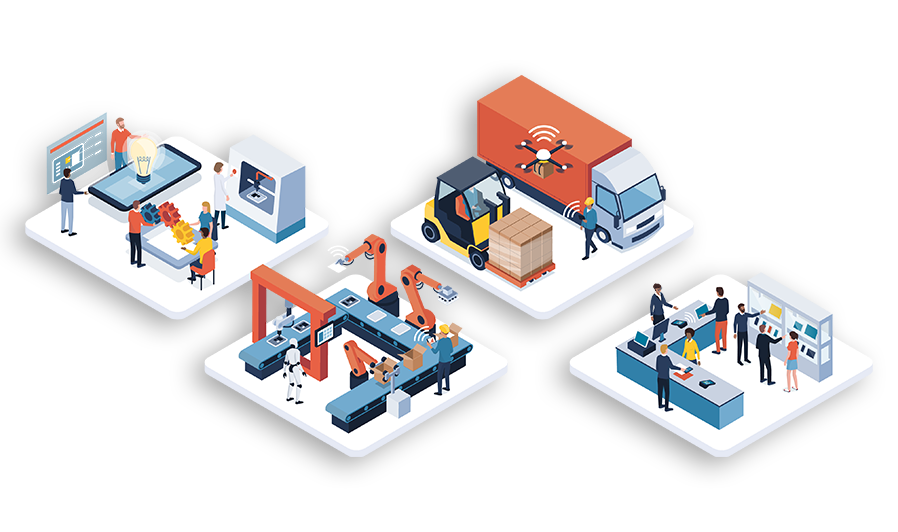
\includegraphics[width=0.6\textwidth]{manufacture}
%		\caption{Minh họa mô hình sản xuất và bán hàng}
%	\end{center}
%\end{figure}
\subsection{Yêu cầu tính năng}
Các tính năng yêu cầu có thể được liệt kê ra như sau:
\begin{itemize}
\item Đăng nhập, đăng xuất, đăng ký, quên mật khẩu.
\item Quản lý các thông tin liên quan đến sản phẩm và bài viết.
\item Yêu cầu đối tác liên kết thông tin với nhau. Chấp nhận liên kết hoặc xóa.
\item Khách hàng có thể xem và đặt sản phẩm ở các trang khác nhau.
\item Có trang quản trị chung cho các nhà bán hàng xem đơn đặt hàng trên trang thương mại điện tử của họ.
\item Nhà bán hàng có thể gửi thư điện tử cho những người có liên kết bạn bè.
\item Hệ thống có thể gửi thư điện tử thông báo đơn hàng.
\item Yêu cầu mở tài khoản cho nhà bán hàng nhanh và tự động. Hạn chế sự can thiệp về mặt kỹ thuật của nhà phát triển.
\item Yêu cầu đo lường được hoạt động của người dùng hệ thống.
\item Sản phẩm có thể có nhiều thuộc tính tùy chọn khi mua hàng.
\item Có thể cài đặt hiển thị số lượng tồn kho của sản phẩm trên trang.
\item Có thể tự tùy chỉnh hầu hết các nội dung trên trang ngoại trừ các chỉnh sửa về mặt đồ họa, giao diện, bố cục của trang.
\end{itemize}
\subsection{Yêu cầu giao diện}
\begin{itemize}
\item Giao diện cần được thiết kế hiện đại và dễ sử dụng.
\item Tương thích ít nhất 80\% các loại màn hình.
\item Mức độ hoàn thiện tương thích màn hình ít nhất 70\%.
\item Thao tác nút bấm to rõ và hạn chế bị giật khi tải lại các thành phần của trang.
\item Tăng các thành phần phản ứng với hành động của người dùng để tạo cảm giác hệ thống đang xử lý liền mạch không bị chậm chạp.
\end{itemize}
\subsection{Yêu cầu hiệu suất}
\begin{itemize}
\item Tất cả các tương tác của người dùng không được phản hồi chậm quá 3 giây.
\item Tất cả phản hồi có thể đợi quá 5 giây cần được phản hồi lại tiến độ hoàn thành. Hoặc tình trạng truy vấn.
\item Các thay đổi dữ liệu không được cập nhật chậm hơn 5 phút sau khi sửa đổi.
\end{itemize}

\subsection{Yêu cầu thiết kế}
\begin{itemize}
\item Hệ thống sử dụng các công nghệ còn được duy trì và phát triển.
\item Hệ thống có thể chia nhỏ ra thành các đội nhóm khi trở nên quá lớn.
\item Hệ thống có thể nâng cấp theo chiều ngang với các lựa chọn có chi phí hợp lý.
\item Hệ thống không bị phụ thuộc và có phương pháp phát triển dự phòng.
\end{itemize}

\subsection{Yêu cầu phi tính năng}
\begin{itemize}
\item Mã hóa thông tin mật khẩu.
\item Sao lưu dự phòng dữ liệu hằng tháng.
\item Sao lưu dự phòng tiến trình thực thi ổn định.
\end{itemize}

\subsection{Vai trò}
\subsubsection{Người bán hàng}
Người bán hàng là người có quyền công bố dữ liệu của họ cho mọi người truy cập thông qua một tên miền cụ thể.

Người bán hàng có thể mời người bán hàng khác, gộp dữ liệu sản phẩm của họ vào bày bán ở trang của mình. Hoặc cũng có thể tham giam đóng góp sản phẩm của mình vào các sàn bán hàng của những người bán hàng khác.

\subsubsection{Người mua hàng}
Người mua hàng là người thực hiện các hoạt động xem thông tin, tạo giỏ hàng, thêm sản phẩm vào giỏ hàng và đặt mua. Người mua hàng không cần thiết phải đăng nhập vào hệ thống. Chỉ cần để lại thông tin địa chỉ để giao hàng là được. Vì hiện tại, hai hình thức thanh toán chuyển khoản và thanh toán \acrshort{cod} rất an toàn cho người bán. Nếu có rủi ro thì chi phí vận chuyển là không quá lớn.

Người mua hàng nếu chủ động lưu trữ thông tin đơn hàng hoặc các hoạt động để cá nhân hóa dữ liệu thì có thể đăng nhập trước khi thực hiện các thành động liên quan.

\subsection{Hoạt động}
Giống như các hệ thống khác, hoạt động được chia ra thành tạo, xem, sửa, xóa. Các hoạt động này được xác định là xảy ra ở tên miền nào, dữ liệu đối tượng gì, do ai có vai trò gì thực hiện.

Với cách xác định hoạt động như trên, có gần với khái niệm \emph{phương thức} của đối tượng trong quan niệm thiết kế hướng đối tượng.

\subsection{Phân quyền}

Phân quyền không chỉ giúp cho hệ thống trở nên bảo mật hơn. Mà còn giúp cho đội ngũ phát triển làm việc chặt chẽ hơn với dữ liệu. Một dạng dữ liệu được phân quyền với yêu cầu đặc tả của khách hàng không thể truyền đạt hết cho tất cả những thành viên trong nhóm được. Điều đó gây ra các lỗ hổng đằng sau \gls{controller} trong mô hình \acrshort{mvc}. Hệ thống sử dụng các nút xử lý mang theo thông tin chung đại diện cho người truy cập. Trong đó có thể phân tách định nghĩa được hoạt động và phân quyền được chặt chẽ hơn. Dưới đây là một số định nghĩa về phân quyền cần lưu ý:

\subsubsection{Quyền đại diện}\label{what-is-owner}
Khi thực hiện truy vấn dữ liệu, cần xác định nguồn gốc của truy vấn đến từ \gls{request} nào \cite{http}. Quyền đại diện cho truy vấn được cấp cho tài khoản nhà bán hàng có tên miền khớp với tên miền chứa trong \gls{request} đó. Tức là có thể lấy được ID của tài khoản đại diện cho \gls{request} hiện tại. 

Chỉ có tài khoản người bán hàng mới có thể đại diện cho một truy vấn. Khi người bán hàng truy vấn từ một trang không phải thuộc sở hữu của họ. Thì hệ thống thay vì căn cứ vào tên miền ở trong \gls{request} hiện tại như cách cũ, nó sẽ trả về luôn \gls{id} của người bán hàng hiện tại. Tức là ghi đè quyền đại diện nếu người thực hiện truy vấn là một nhà bán hàng.

Quyền đại diện thường được sử dụng để xem dữ liệu như một nhà bán hàng tại một tên miền cụ thể. Nghĩa là khi người dùng truy vấn dữ liệu sản phẩm tại một domain nào đó. Thì hệ thống sẽ hỏi cơ sở hữu liệu ai đại diện cho truy vấn này để trả về dữ liệu tương ứng cho truy vấn đó.

Điều này cho phép cùng một hệ thống máy chủ giao diện khi cài đặt với các tên miền khác nhau sẽ trả về các kết quả khác nhau.

Phân quyền này dựa trên chứng thực \gls{headers} của \gls{request}. Tức là nếu ở ứng dụng \gls{mobile} hoặc một nền tảng khác không chứng thực được \gls{headers}. Người dùng không thể giả mạo \gls{headers} để truy vấn thông tin của nhà bán hàng.

Nội dung và phương pháp chứng thực \gls{headers} \gls{request} nằm ngoài phạm vi đề cập của đồ án.

\subsubsection{Quyền hành động}

\textbf{Quyền sở hữu.} Đối với quyền sở hữu. Ai tạo ra dữ liệu thì người đó mới có quyền xóa dữ liệu đó. Cho nên tất cả các bảng đều phải có ghi thông tin người tạo. Bởi vì trong quá trình phát triển đồ án theo yêu cầu thực tế, mối liên hệ giữa các bảng có thể thay đổi nhưng quyền sở hữu giữa dữ liệu đó và người sở hữu không thay đổi. Nếu tạo ra dữ liệu mà không đăng nhập, không xác định được người sở hữu, thì dữ liệu sẽ thuộc về người đại diện cho truy cập (Xem chi tiết người đại diện của truy cập mục \ref{what-is-owner}).

\textbf{Chuyển quyền sở hữu.} Khi tạo đơn đặt hàng, tạo nội dung, dữ liệu sản phẩm cho người khác. Phải quyển quyền sở hữu sau đó. Sẽ có nghiệp vụ chạy ngầm để xét duyệt và ghi đè quyền sở hữu cho người thừa kế. Ghi thông tin người tạo vào dữ liệu vào một trường khác nếu cần. Nhưng bản chất dữ liệu đó đã chuyển quyền sở hữu rồi.

Nghĩa là, coi như người thừa kế (\emph{người được chuyển}) tạo ra dữ liệu đó. sau khi chuyển người sở hữu cũ không có quyền xóa nữa.

\textbf{Quyền xem.}\label{read:permission} đa dạng hơn tùy trường hợp sử dụng.

Quyền xem được thiết đặt theo thứ tự: mặc định, bảng dữ liệu, trường dữ liệu. Nếu định nghĩa quyền xem cho một bảng dữ liệu cụ thể, thì hệ thống sẽ thực hiện định nghĩa đó thay cho quyền mặc định. Tương tự, nếu một trường có định nghĩa quyền xem cho riêng nó, thì khi truy vấn bảng dữ liệu, định nghĩa quyền chỉ áp dụng cho của bảng. Sau đó nếu truy cập hợp lệ vào trường đó thì mới trả về được dữ liệu của trường.

Ví dụ cho trường hợp phân quyền cho trường dữ liệu là khi truy vấn đến bảng người dùng, người xem có thể xem tên, hình ảnh đại diện nhưng không thể xem số điện thoại và mật khẩu đã mã hóa.

Quyền xem chia ra làm hai loại là phân quyền trực tiếp và phân quyền gián tiếp.

\begin{itemize}
\item Đối với phân quyền trực tiếp thì người tạo ra, người sở hữu dữ liệu toàn quyền xem với dữ liệu đó.
\item Quyền xem gián tiếp là quyền cấp cho người xem dữ liệu mà không cần đăng nhập, hoặc đăng nhập nhưng không phải là nhà bán hàng.

Người xem gián tiếp được định nghĩa là khi truy cập dữ liệu dưới một tên miền, thì thông qua tên miền để lấy được quyền truy cập đến các dữ liệu được chia sẻ của: người sở hữu tên miền và người chia sẻ dữ liệu cho tên miền. Hoặc có thể hiểu là người mua hàng đã thông qua tên miền để truy cập đến dữ liệu của nhà bán hàng. Hoặc ngược lại căn cứ theo tên miền tìm nhà bán hàng đại diện để phục vụ dữ liệu cho người dùng.

\end{itemize}

\textbf{Quyền tạo} Khi tạo dữ liệu, đối với một số bảng dữ liệu bắt buộc đăng nhập thì người dùng phải đăng nhập, hoặc là nhà bán hàng thì mới có thể tạo.

Cũng có trường hợp các loại dữ liệu không cần đăng nhập vẫn tạo được để tạo ra sự thuận tiện cho người mua hàng. Ví dụ thêm một sản phẩm vào giỏ hàng. Thực tế khi mua hàng tại các siêu thị, người mua hàng có thể yêu cầu mở thẻ thành viên hoặc là không.

Những dữ liệu không đăng nhập có thể xem bởi tất cả mọi người, nhưng những sản phẩm có thông tin người tạo cần được xem xét cho phép truy cập bởi một số người liên quan chẳng hạn như đơn hàng được tạo trên cửa hàng. Người chủ cửa hàng cần quyền xem đơn hàng đó.


\subsubsection{Dưới đây là các mô tả cụ thể hơn về phân quyền:}

\textbf{Người dùng} Người dùng có thể nhìn thấy thông tin cá nhân cơ bản của chính họ và của những người đã chấp nhận bạn bè.

\textbf{Lời mời kết bạn} Người tạo ra lời mời và người được mời có thể nhìn thấy lời mời đó.

\textbf{Hợp đồng} Hợp đồng tương tự như lời mời kết bạn chỉ người tạo ra và đối tác của người đó được xem dữ liệu.

\textbf{Các tương tác} Các tương tác được xem công khai cho tất cả mọi người nhưng chỉ người tạo ra mới được chỉnh sửa.

\textbf{Thông báo} Thông báo từ hệ thống đến người dùng chỉ được xem bởi chính người đó. Trong trường hợp gửi thông báo cho nhau thì người gửi và người nhận được xem thông báo đó.

\textbf{Nhóm} Nhóm được xem bởi người tham gia nhóm và người đã chấp nhận lời mời tham gia nhóm. Lời mời tham gia nhóm tương tự với lời mời kết bạn.

\textbf{Thống kê truy cập} Thống kê theo dõi truy cập của một cá nhân chỉ được truy cập quản lý bởi chính cá nhân đó.

\textbf{Các bảng công việc} Khi giữa các tài khoản người dùng và tài khoản nhà bán hàng có kí hợp đồng lao động, người dùng có thể tạo bảng để chấm công khi làm việc cho một nhà bán hàng nào đó. Nên nhà bán hàng và người chấm công có thể xem. Yêu cầu chốt công tạo ra bởi người chấm công nhưng không ai có thể xóa. Nhà bán hàng có thể cập nhật hoặc ghi chú vào bảng chốt công.

\textbf{Thông tin công khai} Các thông tin công khai là những thông tin được tạo ra bởi nhà bán hàng và công khai truy cập thông qua một tên miền cụ thể. Đối với các truy cập không có thông tin tên miền. Người dùng đó không có quyền truy cập vào dữ liệu công khai. Ngoại trừ trường hợp người dùng đó đăng nhập với tài khoản nhà bán hàng (xem thêm \textbf{quyền xem} tại mục \ref{read:permission}).

	\fontsize{13px}{13px}\selectfont\justifying

\section{Phân tích, thiết kế}\label{section:readme}
	\begin{figure}[h!]\fontsize{13px}{13px}\selectfont
		\begin{center}	
			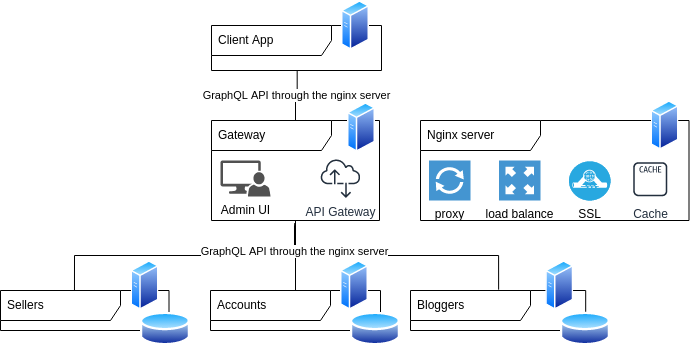
\includegraphics[width=\textwidth]{srs}
			\caption{Thiết kế chung của hệ thống}
		\end{center}
	\end{figure}
	Hệ thống thiết kế hướng dịch vụ chia làm 3 dịch vụ nhỏ là: sellers, accounts và bloggers. Tại máy chủ gateway có nhiệm vụ phân tích truy vấn đồ thị thành nhiều đồ thị con và gửi đến các dịch vụ xử lý. Sau đó gộp kết quả lại và trả về cho truy vấn. Gateway đồng thời cũng cung cấp giao diện quản lý chung cho tất cả các dịch vụ.
	
	Giao tiếp giữa các máy chủ dịch vụ thực hiện thông qua phương thức \acrshort{http}. Sử dụng máy chủ web nginx để liên kết cổng. Đồng thời thực hiện các chức năng chứng thực, phân phối tải,...
	\fontsize{13px}{13px}\selectfont\justifying

\subsection{Sơ đồ ca sử dụng}
% https://www.uml-diagrams.org/use-case-diagrams.html
\subsubsection{Tính năng tổng quát}
\begin{figure}[hbt!]\fontsize{13px}{13px}\selectfont
	\centering
	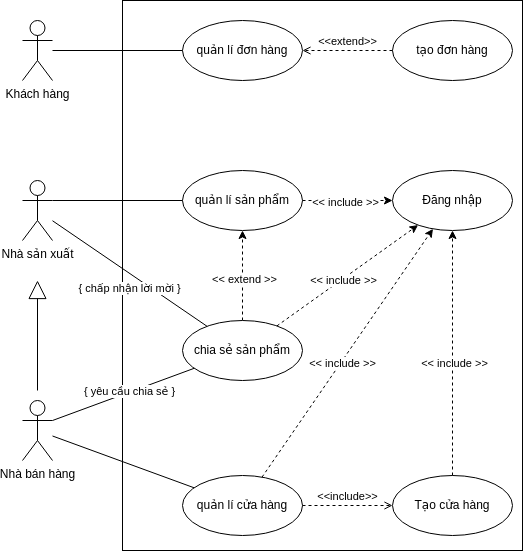
\includegraphics[width=0.8\textwidth]{usecase-usecase}
	\caption{Sơ đồ ca sử dụng tổng quát}
	\justifying
	Khách hàng có thể đặt hàng và xem đơn hàng vừa đặt mà không cần đăng nhập. Nhà sản xuất có thể mở tài khoản để đăng tải thông tin về doanh nghiệp cũng như sản phẩm của mình. Sau đó chia sẻ cho các nhà bán hàng để phân phối thông tin này đến các nhà bán hàng.
\end{figure}
\clearpage
\subsubsection{Tính năng đăng nhập}
\begin{figure}[hbt!]\fontsize{13px}{13px}\selectfont
\centering
		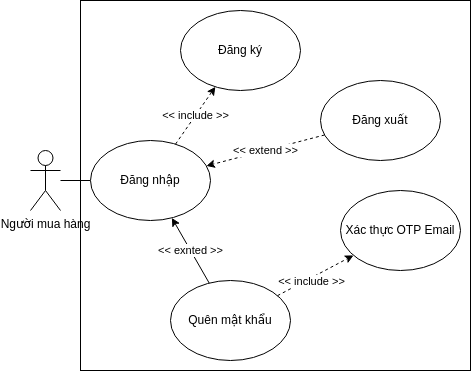
\includegraphics[width=0.7\textwidth]{usecase-login}
		\caption{Sơ đồ ca đăng nhập}
\justifying
Chức năng đăng nhập bao gồm tính năng đăng ký. Trong trường hợp quên mật khẩu, người dùng có thể xác thực đặt lại thông tin mật khẩu thông qua hộp thư điện tử.
\end{figure}

\subsubsection{Tính năng quản lí sản phẩm}
\begin{figure}[hbt!]\fontsize{13px}{13px}\selectfont
\centering
		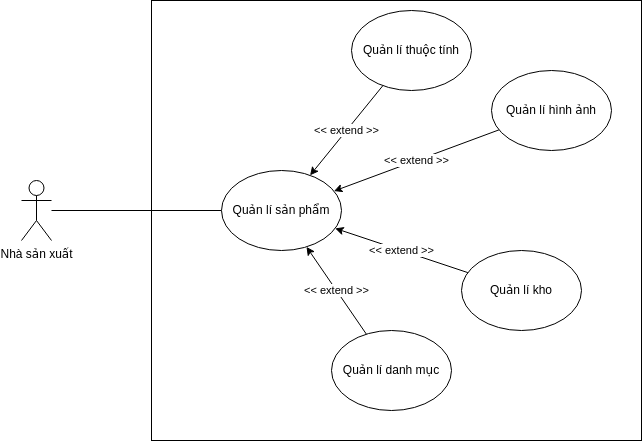
\includegraphics[width=0.6\textwidth]{usecase-sellers}
		\caption{Sơ đồ ca quản lí sản phẩm}
\justifying
Quản lí sản phẩm bao gồm tất cả các tính năng liên quan phục vụ cho việc đăng tải thông tin sản phẩm. Bao gồm thông tin tồn kho của sản phẩm đó.
\end{figure}

\subsubsection{Tính năng chia sẻ sản phẩm}
\begin{figure}[hbt!]\fontsize{13px}{13px}\selectfont
\centering
		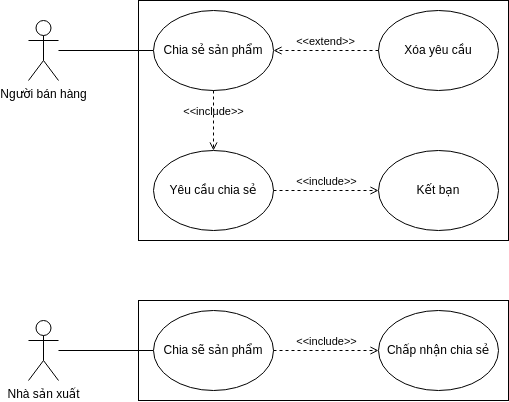
\includegraphics[width=0.6\textwidth]{usecase-contract}
		\caption{Sơ đồ ca yêu cầu chia sẻ}
\justifying
Tính năng chia sẻ sản phẩm giúp cho nhà sản xuất đăng tải, phân phối thông tin của họ trên các trang của nhà bán hàng. Tính năng này yêu cầu sử dụng tính năng kết bạn trước đó.
\end{figure}

\subsubsection{Tính năng kết bạn}
\begin{figure}[hbt!]\fontsize{13px}{13px}\selectfont
\centering
		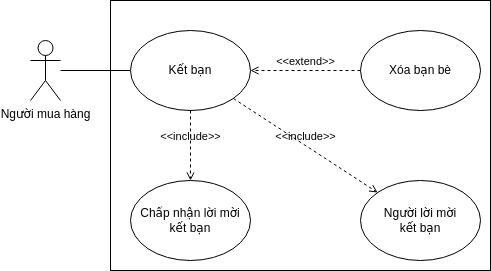
\includegraphics[width=0.6\textwidth]{usecase-relationship}
		\caption{Sơ đồ ca trường hợp kết bạn}
\justifying
Tính năng kết bạn yêu cầu người dùng phải biết username của nhau trước đó. Thông qua username, giữa hai người có thể gửi lời mời kết bạn cho nhau hoặc xác nhận.
\end{figure}

\clearpage
\subsubsection{Tính năng quản lí cửa hàng}
\begin{figure}[hbt!]\fontsize{13px}{13px}\selectfont
\centering
		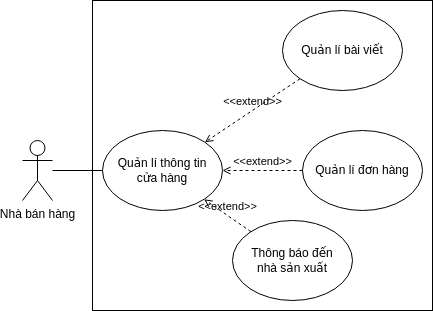
\includegraphics[width=0.5\textwidth]{usecase-store}
		\caption{Sơ đồ ca trường hợp quản lí cửa hàng}
\justifying
Với tính năng quản lí cửa hàng, nhà bán hàng có thể chỉnh sửa thông tin của cửa hàng. Ví dụ như cài đặt màu thương hiệu, tên cửa hàng, slogan, mã số doanh nghiệp,... Các đơn hàng được đặt trên trang sẽ thuộc về người nhà bán hàng.
\end{figure}

\subsubsection{Tính năng đặt hàng}
\begin{figure}[hbt!]\fontsize{13px}{13px}\selectfont
\centering
		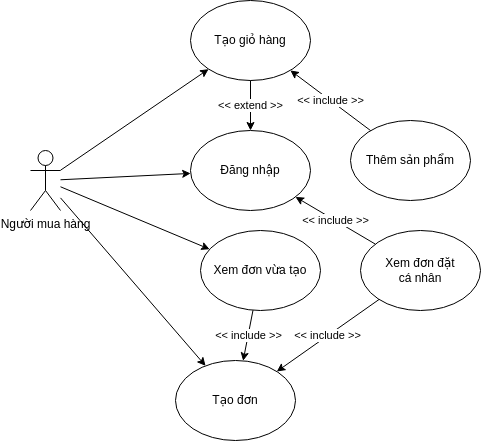
\includegraphics[width=0.7\textwidth]{usecase-order}
		\caption{Sơ đồ ca đặt hàng}
\justifying
Tính năng đặt hàng giúp người mua hàng để lại thông tin mua hàng bao gồm địa chỉ nhận hàng và thông tin số lượng thuộc tính của từng sản phẩm đặt mua. Sử dụng tính năng đặt hàng cũng đồng thời gửi thông báo đến người sở hữu cửa hàng về thông tin đơn hàng.
\end{figure}

% Tính năng chia sẻ là khi lời mời được chấp nhận, sản phẩm của trang thương mại điện tử này có thể hiển thị và đặt mua ở trên trang khác. Nếu có cập nhật thì sản phẩm sẽ tự động đồng bộ.

\clearpage
\subsubsection{Tính năng thông báo}
\begin{figure}[hbt!]\fontsize{13px}{13px}\selectfont
\centering
		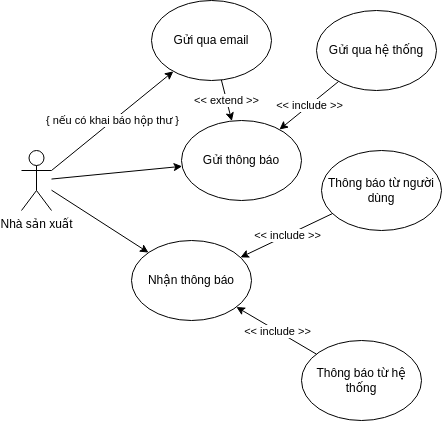
\includegraphics[width=0.8\textwidth]{usecase-notification}
		\caption{Sơ đồ ca trường hợp thông báo}
\justifying
Tính năng thông báo giúp nhà bán hàng gửi thông báo cho nhà sản xuất hoặc ngược lại. Đồng thời, thông qua tính năng này. Hệ thống có thể gửi thông báo đơn hàng đến nhà bán hàng khi có đơn hàng được tạo.

Thông báo chia làm hai loại là thông báo hệ thống và thông báo thư điện tử. Thông báo hệ thống sẽ gửi đến giao diện hệ thống của người nhận. Thông báo thư điện tử sẽ thực hiện chức năng giống hệt như hành động gửi thư điện tử thông thường nhưng khác ở chỗ các thông tin thư sẽ được lưu trữ và hiển thị một phần trên giao diện của hệ thống.
\end{figure}
	\fontsize{13px}{13px}\selectfont\justifying

\clearpage
\subsection{Sơ đồ hoạt động}
% https://www.uml-diagrams.org/activity-diagrams.html
\begin{figure}[h]\fontsize{13px}{13px}\selectfont
	\centering
	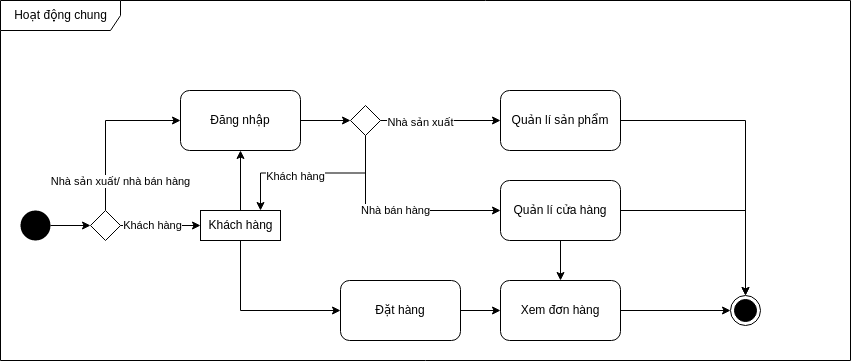
\includegraphics[width=\textwidth]{activity}
	\caption{Sơ đồ hoạt động tổng quát}
	\justifying
	Hoạt động tổng quát của hệ thống bao gồm các hành động mua hàng của khách hàng. Khách hàng mua hàng có thể đăng nhập hoặc không. Hoạt động quản lý sản phẩm, các thông tin khác của nhà sản xuất yêu cầu hoạt động đăng nhập trước đó.
\end{figure}


\begin{figure}[h!]\fontsize{13px}{13px}\selectfont
	\begin{center}	
		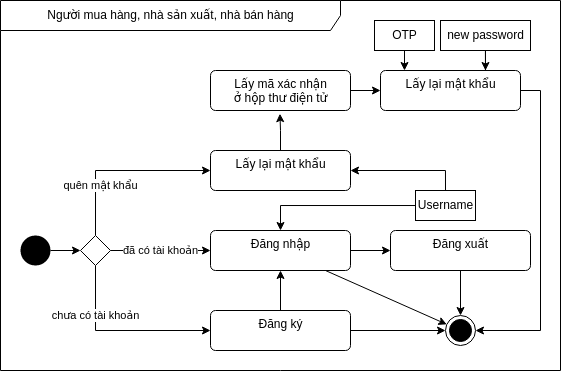
\includegraphics[width=0.8\textwidth]{activity-login}
		\caption{Sơ đồ hoạt động đăng nhập}
	\end{center}
\end{figure}


\begin{figure}[t]\fontsize{13px}{13px}\selectfont
\centering
		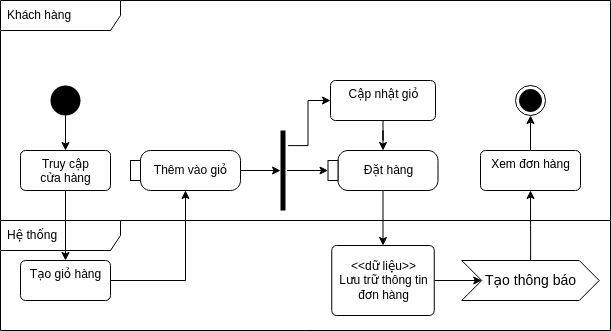
\includegraphics[width=0.7\textwidth]{activity-order}
		\caption{Sơ đồ hoạt động đặt hàng}
\justifying
Hoạt động đặt hàng được thực hiện ở phía máy khách. Khách hàng thông qua trình duyệt để thực hiện mua hàng. Hệ thống được đề cập trong sơ đồ nghĩa là phần mã javascript hoạt động dưới nền khi người dùng sử dụng trang web.
\end{figure}
\begin{figure}[btp]\fontsize{13px}{13px}\selectfont
	\begin{center}	
		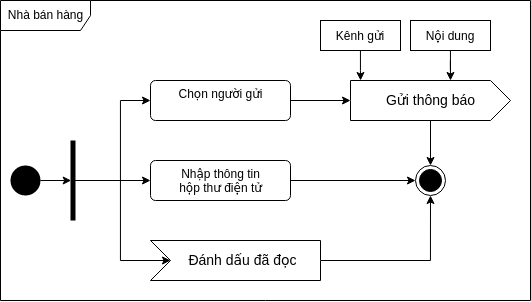
\includegraphics[width=0.7\textwidth]{activity-notification}
		\caption{Sơ đồ hoạt động thông báo}
	\end{center}
\end{figure}


\clearpage
\begin{figure}[t]\fontsize{13px}{13px}\selectfont
	\centering
		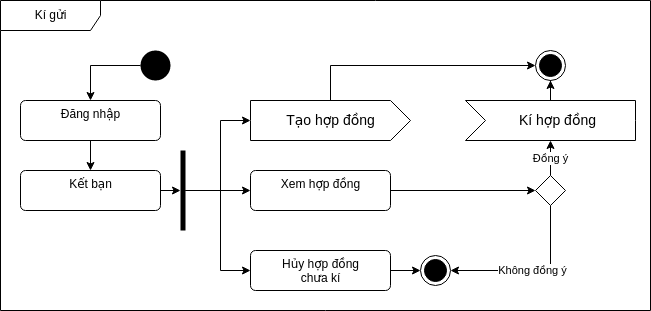
\includegraphics[width=\textwidth]{activity-contract}
		\caption{Sơ đồ hoạt động yêu cầu chia sẻ}
	\justifying
	Sơ đồ hoạt động ký hợp đồng giữa nhà bán hàng và nhà sản xuất. Sơ đồ có đề cập đến hoạt động kết bạn. Hoạt động kết bạn này sẽ được mô tả ở sơ đồ khác. Sau khi hoàn thành hoạt động lý gửi. Nhà bán hàng có thể hiển thị sản phẩm của nhà sản xuất lên trang thương mại điện tử của mình.
\end{figure}

\begin{figure}[h]\fontsize{13px}{13px}\selectfont
\centering
		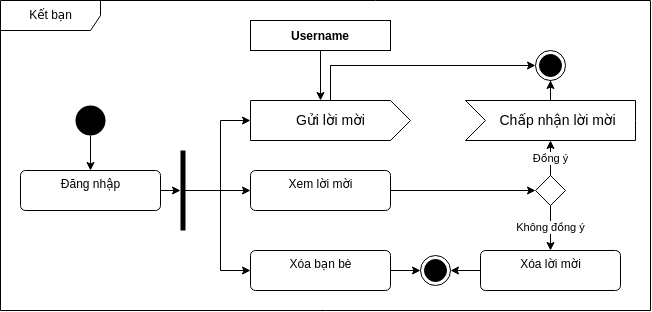
\includegraphics[width=\textwidth]{activity-relationship}
		\caption{Sơ đồ hoạt động kết bạn}
\justifying
Sau khi hoàn thành hoạt động kết bạn, nhà bán hàng có thể gửi lời mời chia sẻ sản phẩm đến các nhà sản xuất khác. Hoạt động gửi lời mời kết bạn có phân biệt người gửi và người nhận nhưng không hiển thị điều này trên giao diện.
\end{figure}

	\fontsize{13px}{13px}\selectfont\justifying

\subsection{Sơ đồ tuần tự}

% https://www.uml-diagrams.org/sequence-diagrams.html
\FloatBarrier
\begin{figure}[h]\fontsize{13px}{13px}\selectfont
	\begin{center}	
		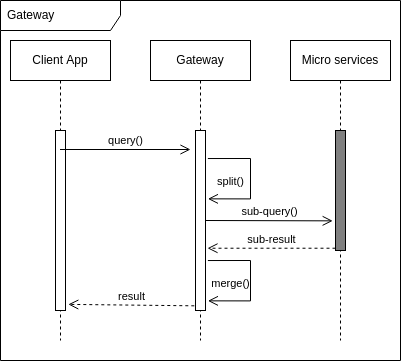
\includegraphics[width=0.8\textwidth]{sequence-gateway}
		\caption{Sơ đồ tuần tự hoạt động của gateway}
	\end{center}

Giải thích:
\begin{enumerate}[before=\fontsize{13px}{13px}\selectfont]
	\item Một truy vấn đồ thị từ ứng dụng khách sẽ gửi đến gateway.
	\item Gateway sẽ phân tích ra thành các đồ thị con cho các máy chủ dịch vụ tương ứng
	\item Các máy chủ dịch vụ nhận và thực hiện các tuy vấn với cơ sở dữ liệu.
	\item Khi nhận được dữ liệu từ các máy chủ dịch vụ, gateway sẽ gộp lại và gửi cho ứng dụng khách.
\end{enumerate}
\end{figure}

\clearpage
\FloatBarrier
\begin{figure}[!htbp]\fontsize{13px}{13px}\selectfont
	\begin{center}	
		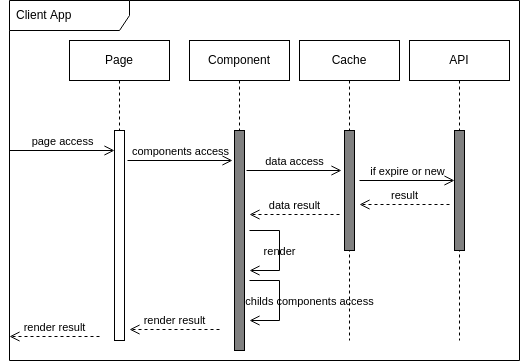
\includegraphics[width=\textwidth]{sequence-component}
		\caption{Sơ đồ tuần tự kết xuất giao diện}
	\end{center}
Giải thích:
\begin{enumerate}[before=\fontsize{13px}{13px}\selectfont]
	\item Người dùng truy cập vào trang của ứng dụng khách.
	\item Trang sẽ truy cập đến components của cấu trúc react.js
	\item Khi component được kết xuất thành công sẽ gọi lấy dữ liệu từ bộ nhớ cache
	\item Bộ nhớ cache thông qua truy vấn từ component sẽ sử dụng làm cache-key để lấy dữ liệu cũ hoặc gọi dữ liệu mới từ máy chủ.
	\item Kết quả trả về lại cho component tái kết xuất.
	\item Khi kết xuất nếu có gọi đến component con thì tiếp tục quá trình 2
	\item Sau quá trình kết xuất hoàn tất thì trả dữ liệu cho màn hình hiển thị.
\end{enumerate}
\end{figure}

\clearpage
\FloatBarrier
\begin{figure}[!htbp]\fontsize{13px}{13px}\selectfont
	\begin{center}	
	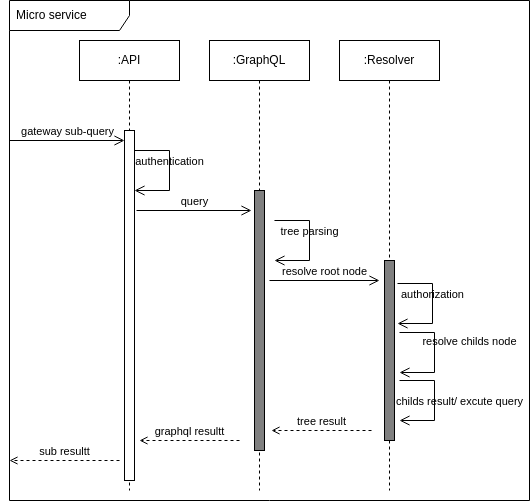
\includegraphics[width=0.8\textwidth]{sequence-service}
	\caption{Sơ đồ tuần tự xử lí truy vấn}
		\end{center}
	Giải thích:
	\begin{enumerate}[before=\fontsize{13px}{13px}\selectfont]
		\item Một truy vấn từ Gateway đến máy chủ dịch vụ sẽ được định danh tại lớp API.
		\item Sau đó nội dung truy vấn sẽ được gửi đến lớp GraphQL.
		\item Lớp GraphQL đóng gói truy vấn thành một cây dữ liệu và gửi cho lớp Resolver giải quyết.
		\item Lớp Resolver quét qua tất cả các nút và quy nạp kết quả.
		\item Dữ liệu được trả về cho GraphQL và tiếp tục trả cho lớp API để phản hồi cho máy chủ gateway.
	\end{enumerate}
\end{figure}


	\fontsize{13px}{13px}\selectfont\justifying

\subsection{Sơ đồ thành phần}

\begin{figure}[h!]\fontsize{13px}{13px}\selectfont
\centering
		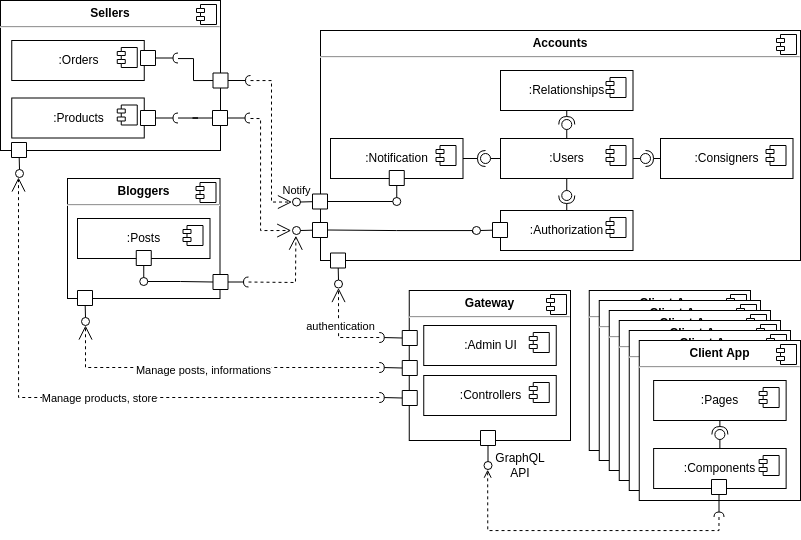
\includegraphics[width=\textwidth]{component}
		\caption{Sơ đồ thành phần hệ thống}
\justifying
Các ứng dụng phía máy khách giao tiếp với hệ thống máy chủ thông qua máy chủ trung tâm là gateway. Gateway sử dụng các dịch vụ quản lí của các máy chủ dịch vụ. Đối với máy chủ dịch vụ accounts, máy chủ gateway sử dụng chức năng authentication trả về cookie hoặc token cho ứng dụng máy khách.

Máy chủ dịch vụ sellers sử dụng chức năng gửi thông báo và chức năng lấy vai trò người dùng hiện tại của accounts. Nghĩa là khi một hành động mang theo \acrshort{headers} sellers căn cứ vào đó yêu cầu đến máy chủ dịch vụ accounts để biết được, ai là người đại diện cho truy vấn và ai là những người đóng góp cho người đại diện đó. Từ đó, sellers có thể căn cứ để trả về danh sách sản phẩm đúng với yêu cầu.
\end{figure}
	\fontsize{13px}{13px}\selectfont\justifying

\subsection{Sơ đồ triển khai}
\begin{figure}[h!]\fontsize{13px}{13px}\selectfont
\centering
		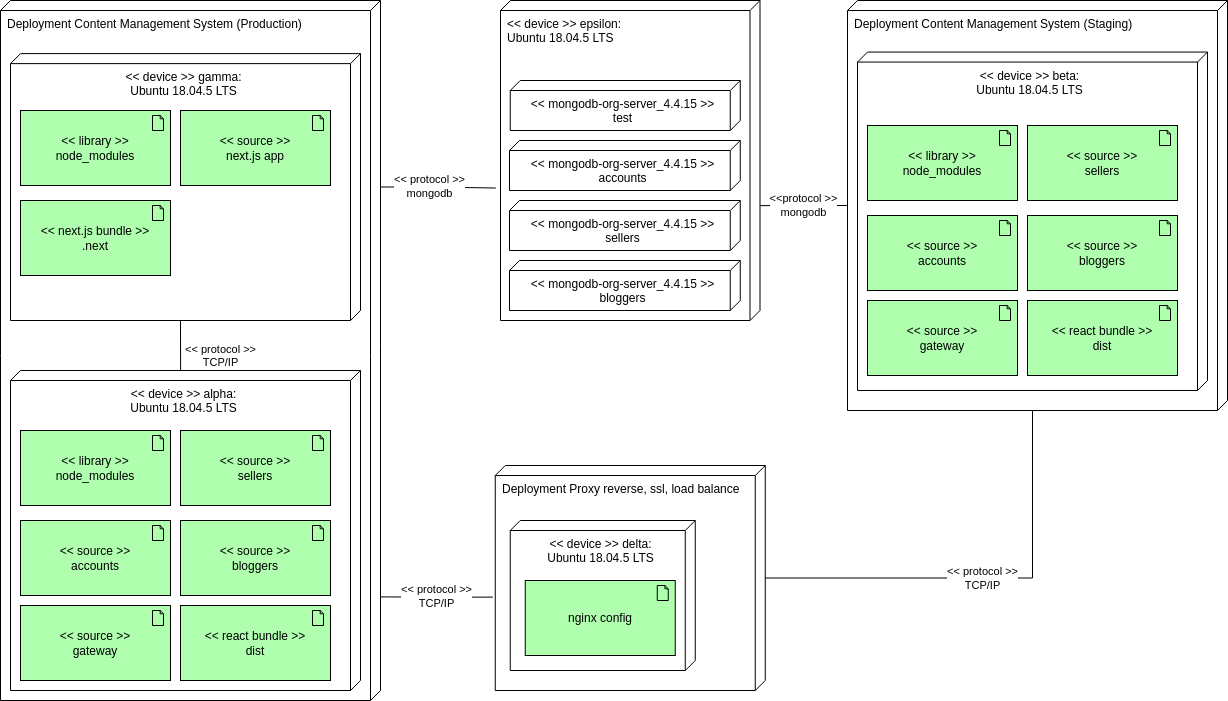
\includegraphics[width=\textwidth]{deployment}
		\caption{Sơ đồ triển khai tổng quát}
\justifying
Hệ thống cần tối thiểu 4 môi trường phát hành khác nhau. Trong môi trường \Gls{production} và môi trường \Gls{staging}, các thiết bị có thể nhân bản ra để phục vụ việc cân bằng tải thông qua thuật toán phân phối tải của máy chủ nginx.

Hệ thống sử dụng CI/CD của Github Actions giúp cho việc triển khai trở nên tự động và có thể sao lưu dự phòng tại mỗi phiên bản phát hành.

Github Actions cơ bản cung cấp chức năng kích hoạt đoạn mã triển khai của hệ thống khi có một hoạt động quản lý mã nguồn phù hợp với nội dung mà chúng ta đã cấu hình. Ví dụ như khi mã nguồn được gộp vào nhánh cho tên là \gls{production}, thì chạy mã triển khai \gls{production} ở phía máy chủ.
\end{figure}

	\fontsize{13px}{13px}\selectfont\justifying

\clearpage
\subsection{Sơ đồ lớp}
\FloatBarrier
\begin{figure}[!htbp]\fontsize{13px}{13px}\selectfont
	\centering
	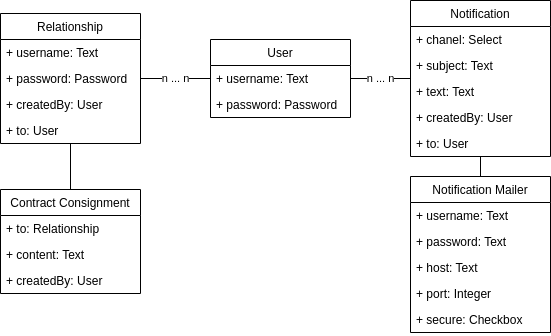
\includegraphics[width=0.8\textwidth]{class-accounts}
	\caption{Sơ đồ lớp quản lý kết bạn và chia sẻ}
	\justifying
	Các lớp thực hiện chức năng đăng nhập, đăng xuất, đăng ký. Gửi lời mời kết bạn, đồng ý kết bạn. Gửi yêu cầu chia sẻ sản phẩm. Thực hiện các chức năng thông báo.
\end{figure}

\FloatBarrier
\begin{figure}[!htbp]\fontsize{13px}{13px}\selectfont
	\centering
	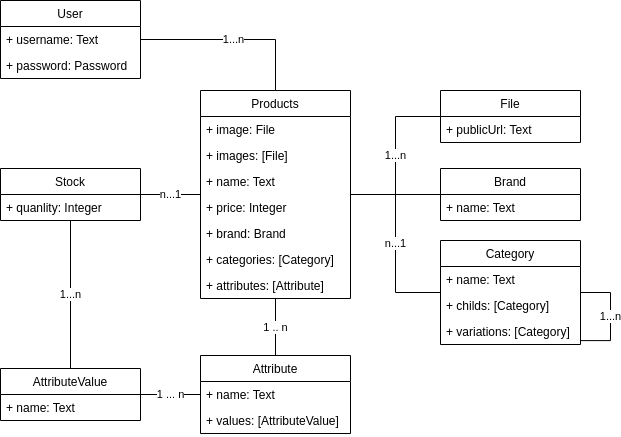
\includegraphics[width=0.8\textwidth]{class-products}
	\caption{Sơ đồ lớp quản lý sản phẩm}
	\justifying
	Các lớp thực hiện chức năng quản lý sản phẩm và tồn kho. Sản phẩm có nhiều thuộc tính và nhóm thuộc tính như màu sắc và kích thước. Đối với từng tổ hợp nhóm thuộc tính sẽ có một số lượng kho tương ứng.
\end{figure}

\clearpage
\FloatBarrier
\begin{figure}[!htbp]\fontsize{13px}{13px}\selectfont
	\centering
	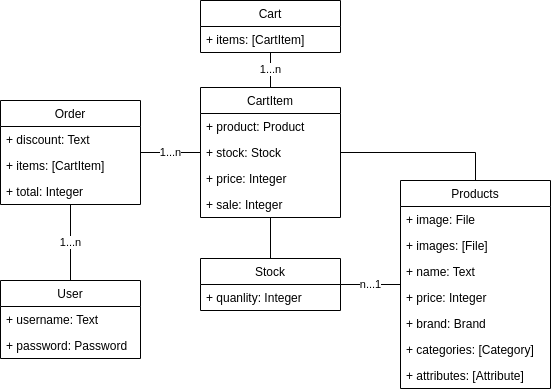
\includegraphics[width=0.8\textwidth]{class-orders}
	\caption{Sơ đồ lớp đặt hàng, quản lý đơn hàng}
\end{figure}
\FloatBarrier
\begin{figure}[!htbp]\fontsize{13px}{13px}\selectfont
	\centering
	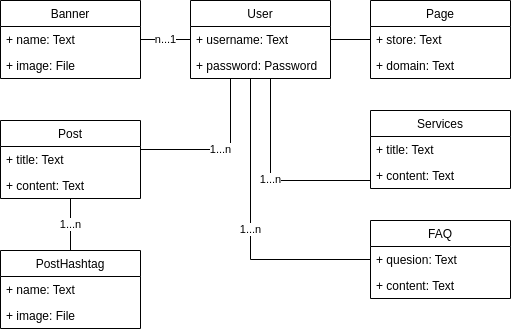
\includegraphics[width=0.8\textwidth]{class-store}
	\caption{Sơ đồ lớp quản lý cửa hàng}
\end{figure}
	\fontsize{13px}{13px}\selectfont\justifying

\subsection{Thiết kế Dữ liệu}
\subsubsection{Bảng ContractConsignment được mô tả như sau}
\begin{table}[!htbp]\fontsize{13px}{13px}\selectfont\justifying
\begin{center}
\caption{Mô tả bảng ContractConsignment.}
\label{table:ContractConsignment}
\begin{tabularx}{0.6\textwidth}{ |l|l|X| } 
\hline
Tên & Kiểu & Mô tả \\
\hline
to & User & Người nhận yêu cầu \\
isAccepted & Checkbox & Tình trạng yêu cầu \\
\hline
\end{tabularx}
\end{center}
\justifying
ContractConsignment sử dụng để gửi yêu cầu chia sẻ được tạo ra bởi nhà bán hàng đến một nhà sản xuất. Cả người tạo và người nhận đều có quyền xóa bản ghi này, kể cả trước hay sau khi chấp nhận.
\end{table}
% ============

\subsubsection{Bảng NotificationMailer được mô tả như sau}
\begin{table}[!htbp]\fontsize{13px}{13px}\selectfont\justifying
\begin{center}
\caption{Mô tả bảng NotificationMailer.}
\begin{tabularx}{0.6\textwidth}{ |l|l|X| } 
\hline
Tên & Kiểu & Mô tả \\
\hline
username & Text & Tên người email \\
password & Text & Mật khẩu email \\
host & Text & hosting \\
port & Integer & cổng \\
secure & Checkbox & secure \\
name & Text & Tên người gửi \\ 
\hline
\end{tabularx}
\label{table:NotificationMailer}
\end{center}
\justifying
Bảng NotificationMailer sử dụng để lưu trữ tài khoản hộp thư điện tử của nhà bán hàng. Tài khoản hộp thư điện tử này dùng để gửi thông báo từ nhà bán hàng cho nhà sản xuất thông qua dịch vụ thư điện tử. Việc này hoàn toàn tương tự với việc gửi thư điện tử thông thường. Khác ở chỗ, nếu sử dụng thông qua hệ thống thì thông tin cơ bản của thư điện tử sẽ được lưu trữ và hiển thị lại màn hình thông báo của hệ thống.
\end{table}
% ============
\clearpage
\subsubsection{Bảng Notification được mô tả như sau}
\begin{table}[!htbp]\fontsize{13px}{13px}\selectfont\justifying
\begin{center}
\caption{Mô tả bảng Notification.}
\begin{tabularx}{0.6\textwidth}{ |l|l|X| } 
\hline
Tên & Kiểu & Mô tả \\
\hline
chanel & Select & Kênh gửi \\
subject & Text & Tiêu đề \\
text & Text & Nội dung \\
seen & Checkbox & Tình trạng \\ 
\hline
\end{tabularx}
\label{table:Notification}
\end{center}
Bảng Notification chứa nội dung thông báo. Tùy chọn kênh thông báo sẽ quyết định cách thông báo được gửi và hiển thị trên hệ thống.
\end{table}
% ============

\subsubsection{Bảng Relationship được mô tả như sau}
\begin{table}[!htbp]\fontsize{13px}{13px}\selectfont\justifying
\begin{center}
\caption{Mô tả bảng Relationship.}
\begin{tabularx}{0.6\textwidth}{ |l|l|X| } 
\hline
Tên & Kiểu & Mô tả \\
\hline
username & Text & Tên người dùng \\
to & Virtual & Người nhận \\
isAccepted & Checkbox & Tình trạng \\
consignment & Virtual & Lời mời \\ 
\hline
\end{tabularx}
\label{table:Relationship}
\end{center}
Bảng Relationship thể hiện một liên kết giữa hai User, không phân biệt người gửi và người nhận. Cả hai đều có quyền xóa liên kết.
\end{table}
% ============
\clearpage
\subsubsection{Bảng User được mô tả như sau}
\begin{table}[!htbp]\fontsize{13px}{13px}\selectfont\justifying
\begin{center}
\caption{Mô tả bảng User.}
\begin{tabularx}{0.6\textwidth}{ |l|l|X| } 
\hline
Tên & Kiểu & Mô tả \\
\hline
username & Text & Tên người dùng \\
password & Password & Mật khẩu \\
phone & Text & Số điện thoại \\
email & Text & Email \\
name & Text & Tên gọi \\
fullname & Text & Tên đầy đủ \\
avatar & File & Ảnh đại diện \\
abount & Text & Thông tin \\
domain & Text & Tên miền \\
isSeller & Checkbox & là nhà sản xuất? \\
forgotAt & DateTime & Quên mật khẩu lúc \\ 
\hline
\end{tabularx}
\label{table:User}
\end{center}
Bảng User sử dụng để lưu trữ thông tin tài khoản. Các chức năng đăng nhập, đăng xuất, đăng ký.
\end{table}
% ============

\subsubsection{Bảng View được mô tả như sau}
\begin{table}[!htbp]\fontsize{13px}{13px}\selectfont\justifying
\begin{center}
\caption{Mô tả bảng View.}
\begin{tabularx}{0.6\textwidth}{ |l|l|X| } 
\hline
Tên & Kiểu & Mô tả \\
\hline
count & Integer & Số lượt xem \\
of & MongoId & Thuộc User \\ 
\hline
\end{tabularx}
\label{table:View}
\end{center}
Bảng view đo lường số lượng người xem đối với một kiểu dữ liệu, số lượng này được lưu trữ tạm và phân tán trên nhiêu máy chủ dịch vụ. Sau một chu kì, các dữ liệu này sẽ được tác vụ chạy ngầm xử lý cộng và ghi vào cơ sở dữ liệu.
\end{table}
% ============
\clearpage
\subsubsection{Bảng Banner được mô tả như sau}
\begin{table}[!htbp]\fontsize{13px}{13px}\selectfont\justifying
\begin{center}
\caption{Mô tả bảng Banner.}
\begin{tabularx}{0.6\textwidth}{ |l|l|X| } 
\hline
Tên & Kiểu & Mô tả \\
\hline
name & Text & tên \\
slogan & Text & slogan \\
image & File & hình ảnh \\
description & Text & mô tả \\
url & Text & đường dẫn \\
type & Select & loại \\
size & Virtual & kích thước \\ 
\hline
\end{tabularx}
\label{table:Banner}
\end{center}
Bảng Banner lưu trữ hình ảnh và các thông tin của hình ảnh để lựa chọn hiển thị trên các không gian khác nhau của trang web.
\end{table}
% ============

\subsubsection{Bảng Contact được mô tả như sau}
\begin{table}[!htbp]\fontsize{13px}{13px}\selectfont\justifying
\begin{center}
\caption{Mô tả bảng Contact.}
\begin{tabularx}{0.6\textwidth}{ |l|l|X| } 
\hline
Tên & Kiểu & Mô tả \\
\hline
phone & Text & số điện thoại \\
name & Text & tên \\
address & Text & địa chỉ \\
email & Text & email \\
note & Text & ghi chú \\
message & Text & tin nhắn \\
isDefault & Checkbox & đánh dấu \\ 
\hline
\end{tabularx}
\label{table:Contact}
\end{center}
Bảng Contact lưu trữ thông tin của khách hàng để lại khi đặt hàng. Đối với các nhà bán hàng không mở tính năng đặt hàng. Sẽ có một biểu mẫu để khách hàng để lại thông tin. Thông tin này cũng được lưu trữ tại bảng Contact.
\end{table}
% ============
\clearpage
\subsubsection{Bảng Page được mô tả như sau}
\begin{table}[!htbp]\fontsize{13px}{13px}\selectfont\justifying
\begin{center}
\caption{Mô tả bảng Page.}
\begin{tabularx}{0.6\textwidth}{ |l|l|X| } 
\hline
Tên & Kiểu & Mô tả \\
\hline
store & Text & Tên cửa hàng \\
logo & File & Ảnh đại diện \\
slogan & Text & Lĩnh vực \\
address & Text & Địa chỉ \\
phone & Text & Số điện thoại \\
email & Text & email \\
intro & Editor & Giới thiệu ngắn \\
contact & Editor & Liên hệ \\
twitter & Text & twitter \\
instagram & Text & instagram \\
pinterest & Text & pinterest \\
youtube & Text & youtube \\
googlePlus & Text & googlePlus \\
googleMap & Text & googleMap \\
zalo & Text & zalo \\
greeting & Text & Lời chào \\
pageId & Text & Facebook pageId \\
pixelId & Text & Facebook pixelId \\
gtag & Text & Google gtag \\
shipMoneySupport & Integer & Hỗ trợ tiền ship \\
ship & Editor & Thông tin ship \\
transfer & Editor & Chuyển khoản \\
color & Color & Màu chủ đạo \\
colorMode & Select & Tông chủ đạo \\
ordering & Checkbox & Cho phép đặt hàng \\
moit & Text & gs1 \\
mst & Text & mã số thuế \\


\hline
\end{tabularx}
\label{table:Page}
\end{center}
Bảng Page hiển thị các thông tin cơ bản của nhà bán hàng. Các thông tin liên hệ và liên kết mạng xã hội.
\end{table}
% ============

\subsubsection{Bảng ProductAttributeValue được mô tả như sau}
\begin{table}[!htbp]\fontsize{13px}{13px}\selectfont\justifying
\begin{center}
\caption{Mô tả bảng ProductAttributeValue.}
\begin{tabularx}{0.6\textwidth}{ |l|l|X| } 
\hline
Tên & Kiểu & Mô tả \\
\hline
value & Text & thuộc tính \\
file & File & hình ảnh mô tả \\ 
\hline
\end{tabularx}
\label{table:ProductAttributeValue}
\end{center}
Giá trị của của thuộc tính sản phẩm được hiểu là tùy chọn cụ thể của một thuộc tính. Ví dụ đối với thuộc tính màu sắc, thì người dùng chọn giá trị thuộc tính là màu đỏ.
\end{table}
% ============

\subsubsection{Bảng ProductAttribute được mô tả như sau}
\begin{table}[!htbp]\fontsize{13px}{13px}\selectfont\justifying
\begin{center}
\caption{Mô tả bảng ProductAttribute.}
\begin{tabularx}{0.6\textwidth}{ |l|l|X| } 
\hline
Tên & Kiểu & Mô tả \\
\hline
label & Text & nhãn \\
name & Text & tên \\
\hline
\end{tabularx}
\label{table:ProductAttribute}
\end{center}
Thuộc tính sản phẩm sẽ được lựa chọn khi người mua hàng thêm sản phẩm vào giỏ hàng. Căn cứ vào thuộc tính sản phẩm và id sản phẩm hiện tại có thể xác định tồn kho của sản phẩm.
Thuộc tính sản phẩm có thể là kích thước, màu sắc,... hoặc là cả thuộc tính và màu sắc.
\end{table}
% ============

\subsubsection{Bảng ProductBrand được mô tả như sau}
\begin{table}[!htbp]\fontsize{13px}{13px}\selectfont\justifying
\begin{center}
\caption{Mô tả bảng ProductBrand.}
\begin{tabularx}{0.6\textwidth}{ |l|l|X| } 
\hline
Tên & Kiểu & Mô tả \\
\hline
name & Text & tên \\
url & Slug & đường dẫn \\
\hline
\end{tabularx}
\label{table:ProductBrand}
\end{center}
ProductBrand hiện thị thương hiệu của sản phẩm. Thương hiệu có thể là chính nhà sản xuất. Hoặc nếu là nhà cung cấp, nhà cung cấp có thể tạo và sử dụng thương hiệu phù hợp với thông tin sản phẩm.
\end{table}
% ============
\clearpage
\subsubsection{Bảng ProductCartItem được mô tả như sau}
\begin{table}[!htbp]\fontsize{13px}{13px}\selectfont\justifying
\begin{center}
\caption{Mô tả bảng ProductCartItem.}
\begin{tabularx}{0.6\textwidth}{ |l|l|X| } 
\hline
Tên & Kiểu & Mô tả \\
\hline
sale & Integer & giá bán \\
price & Integer & giá niêm \\
percent & Virtual & phần trăm \\
isInCart & Virtual & đang trong giỏ \\
quantity & Integer & số lượng \\ 
\hline
\end{tabularx}
\label{table:ProductCartItem}
\end{center}
Chi tiết giỏ hàng được liên kết liệt kê trong giỏ hàng. Các chi tiết giỏ hàng sau khi đặt hàng sẽ được hủy liên kết với giỏ hàng và liên kết với đơn hàng được tạo. Điều này có nghĩa là khi một chi tiết giỏ hàng được tạo. Nó mặc định sẽ có id giỏ hàng. Nếu không có id giỏ hàng thì sẽ có id đơn hàng.
\end{table}
% ============

\subsubsection{Bảng ProductCart được mô tả như sau}
\begin{table}[!htbp]\fontsize{13px}{13px}\selectfont\justifying
\begin{center}
\caption{Mô tả bảng ProductCart.}
\begin{tabularx}{0.6\textwidth}{ |l|l|X| } 
\hline
Tên & Kiểu & Mô tả \\

\hline
contact & MongoId & Liên hệ\\
items & [MongoId] & sản phẩm\\
\hline
\end{tabularx}
\label{table:ProductCart}
\end{center}
Bảng ProductCart lưu trữ thông tin giỏ hàng bao gồm các chi tiết giỏ hàng. ID giỏ hàng được lưu trữ tại localStorage ở các trình duyệt web. Các với cách lưu trữ đơn hàng ở session như một số mô hình khác. Bảng đơn hàng được xem như một bảng bình thường trong cơ sở dữ liệu.
\end{table}
% ============
\clearpage
\subsubsection{Bảng ProductCategory được mô tả như sau}
\begin{table}[!htbp]\fontsize{13px}{13px}\selectfont\justifying
\begin{center}
\caption{Mô tả bảng ProductCategory.}
\begin{tabularx}{0.6\textwidth}{ |l|l|X| } 
\hline
Tên & Kiểu & Mô tả \\
\hline
name & Text & tên \\
description & Editor & mô tả \\
file & File & bìa \\
prioritize & Integer & ưu tiên \\
url & Slug & đường dẫn \\
root & Checkbox & gốc \\
\hline
\end{tabularx}
\label{table:ProductCategory}
\end{center}
Bảng ProductCategory là danh mục để phân loại sản phẩm. Danh mục được biểu diễn như dạng cấu trúc cây. Mỗi nút của cây có thể đánh dấu bao gồm các danh mục tương đương nào. Danh mục tương đương là danh mục không thuộc sở hữu của nhà bán hàng. Nhưng sản phẩm thuộc danh mục tương đương thì cũng thuộc danh mục gốc được đánh dấu.
\end{table}
% ============

\subsubsection{Bảng ProductDiscount được mô tả như sau}
\begin{table}[!htbp]\fontsize{13px}{13px}\selectfont\justifying
\begin{center}
\caption{Mô tả bảng ProductDiscount.}
\begin{tabularx}{0.6\textwidth}{ |l|l|X| } 
\hline
Tên & Kiểu & Mô tả \\
\hline
code & Text & mã \\
type & Select & loại \\
value & Integer & giá trị \\
name & Text & tên \\
description & Text & mô tả \\
condition & Integer & điều kiện \\
image & File & hình ảnh \\
url & Slug & đường dẫn \\
\hline
\end{tabularx}
\label{table:ProductDiscount}
\end{center}
Bảng ProductDiscount lưu trữ thông tin khuyến mãi. Có thể khuyến mãi theo hai hình thức là giảm theo phần trăm hoặc giảm giá cố định. Điều kiện giảm giá có thể có hoặc không và căn cứ theo tổng giá trị đơn hàng.
\end{table}
% ============
\clearpage
\subsubsection{Bảng ProductHashtag được mô tả như sau}
\begin{table}[!htbp]\fontsize{13px}{13px}\selectfont\justifying
\begin{center}
\caption{Mô tả bảng ProductHashtag.}
\begin{tabularx}{0.6\textwidth}{ |l|l|X| } 
\hline
Tên & Kiểu & Mô tả \\
\hline
name & Text & tên \\
url & Slug & đường dẫn \\
\hline
\end{tabularx}
\label{table:ProductHashtag}
\end{center}
Bảng ProductHashtag liên kết với sản phẩm để hiển thị thông tin hashtag của sản phẩm.
\end{table}
% ============

\subsubsection{Bảng ProductOrderStatus được mô tả như sau}
\begin{table}[!htbp]\fontsize{13px}{13px}\selectfont\justifying
\begin{center}
\caption{Mô tả bảng ProductOrderStatus.}
\begin{tabularx}{0.6\textwidth}{ |l|l|X| } 
\hline
Tên & Kiểu & Mô tả \\
\hline
value & Text & giá trị \\
color & Select & màu sắc \\ 
\hline
\end{tabularx}
\label{table:ProductOrderStatus}
\end{center}
Bảng ProductOrderStatus hiển thị trạng thái đơn hàng được đánh dấu để xử lý trong nội bộ của nhà bán hàng.
\end{table}

\subsubsection{Bảng ProductOrder được mô tả như sau}
\begin{table}[!htbp]\fontsize{13px}{13px}\selectfont\justifying
\begin{center}
\caption{Mô tả bảng ProductOrder.}
\begin{tabularx}{0.6\textwidth}{ |l|l|X| } 
\hline
Tên & Kiểu & Mô tả \\
\hline
code & Text & mã \\
isExport & Checkbox & đã xuất \\
payment & Select & hình thức thanh toán \\
saving & Integer & tiết kiệm \\
total & Integer & tổng \\
notification & MongoId & thông báo \\ 
\hline
\end{tabularx}
\label{table:ProductOrder}
\end{center}
Bảng ProductOrder lưu trữ thông tin đặt hàng của khách hàng. Bảng ProductOrder sử dụng lại các chi tiết giỏ hàng trước đó người dùng chọn lưu vào giỏ hàng. Khi bảng ProductOrder được tạo, một thư điện tử với thông tin đặt hàng sẽ được gửi đến nhà bán hàng tương ứng.
\end{table}
% ============
\clearpage
\subsubsection{Bảng ProductStock được mô tả như sau}
\begin{table}[!htbp]\fontsize{13px}{13px}\selectfont\justifying
\begin{center}
\caption{Mô tả bảng ProductStock.}
\begin{tabularx}{0.6\textwidth}{ |l|l|X| } 
\hline
Tên & Kiểu & Mô tả \\
\hline
quantity & Integer & số lượng \\
image & File & hình ảnh \\ 
\hline
\end{tabularx}
\label{table:ProductStock}
\end{center}
Bảng ProductStock lưu trữ thông tin tồn kho của một sản phẩm. Dựa trên thuộc tính được chọn. Một sản phẩm có thể có nhiều bảng tồn kho.
\end{table}
% ============

\subsubsection{Bảng Product được mô tả như sau}
\begin{table}[!htbp]\fontsize{13px}{13px}\selectfont\justifying
\begin{center}
\caption{Mô tả bảng Product.}
\begin{tabularx}{0.6\textwidth}{ |l|l|X| } 
\hline
Tên & Kiểu & Mô tả \\
\hline
image & File & Hình ảnh \\
images & Images & Hình ảnh thêm \\
name & Text & Tên sản phẩm \\
price & Currency & Giá niêm yết \\
sale & Currency & Giá bán \\
percent & Virtual & Phầm trăm giảm giá \\
status & Select & Tình trạng \\
description & Editor & Mô tả \\
detail & File & Chi tiết \\
guide & Editor & Hướng dẫn sử dụng \\
isOutOfStock & Checkbox & Hết hàng \\
sku & Text & sku \\
gs1 & Text & gs1 \\
url & Slug & đường dẫn \\
sold & Virtual & đã bán \\
\hline
\end{tabularx}
\label{table:Product}
\end{center}
Bảng Product hiện thị đầy đủ các thông tin một sản phẩm cần có, Product có rất nhiều quan hệ với các bảng dữ liệu vệ tinh. Đối với một số trường hay được truy vấn. Thay vì tổng hợp và sắp xếp khi truy vấn. Có cách tác vụ chạy ngầm để tính toán và đánh dấu sẵn như tính phần trăm giảm giá, tính sản phẩm này thuộc sản phẩm mới cập nhật hay sản phẩm hết hàng. Ngoài ra, các trường như số lượt xem thay vì thông qua tác vụ chạy ngầm có thể truy vấn ngay khi xử lý và lưu vào bộ nhớ tạm để phản hồi nhanh.
\end{table}
% ============

\subsubsection{Bảng Translate được mô tả như sau}
\begin{table}[!htbp]\fontsize{13px}{13px}\selectfont\justifying
\begin{center}
\caption{Mô tả bảng Translate.}
\begin{tabularx}{0.6\textwidth}{ |l|l|X| } 
\hline
Tên & Kiểu & Mô tả \\
\hline
item & MongoId & item cần dịch \\
listKey & Text & kiểu \\
fieldName & Text & trường dịch \\
lang & Text & ngôn ngữ\\
content & Text & nội dung\\
\hline
\end{tabularx}
\label{table:Translate}
\end{center}
Bảng Translate dùng để dịch cho các trường của một bản ghi bất kì, thuộc kiểu dữ liệu bất kì. Xác định một bảng dịch cần tìm kiếm tất cả các bản dịch cho khóa chính và trường cần dịch.
\end{table}
% ============

\subsubsection{Bảng UploadFile được mô tả như sau}	
\begin{table}[!htbp]\fontsize{13px}{13px}\selectfont\justifying
\begin{center}
\caption{Mô tả bảng UploadFile.}
\begin{tabularx}{0.6\textwidth}{ |l|l|X| } 
\hline
Tên & Kiểu & Mô tả \\
\hline
file & File & tệp \\
address & Text & địa chỉ tệp\\ 
\hline
\end{tabularx}
\label{table:UploadFile}
\end{center}
Bảng UploadFile lưu trữ địa chỉ của tệp sau khi được tải lên và lưu trữ tại máy chủ dịch vụ.
\end{table}

\subsubsection{Bảng UploadImage được mô tả như sau}
\begin{table}[!htbp]\fontsize{13px}{13px}\selectfont\justifying
\begin{center}
\caption{Mô tả bảng UploadImage.}
\begin{tabularx}{0.6\textwidth}{ |l|l|X| } 
\hline
Tên & Kiểu & Mô tả \\
\hline
file & File & tệp \\
alt & Text & mô tả \\ 
\hline
\end{tabularx}
\label{table:UploadImage}
\end{center}
UploadImage lưu trữ địa chỉ của hình ảnh sau khi được tải lên và lưu trữ tại máy chủ dịch vụ.
\end{table}
% ============
\clearpage
\subsubsection{Bảng FAQ được mô tả như sau}
\begin{table}[!htbp]\fontsize{13px}{13px}\selectfont\justifying
\begin{center}
\caption{Mô tả bảng FAQ.}
\begin{tabularx}{0.6\textwidth}{ |l|l|X| } 
\hline
Tên & Kiểu & Mô tả \\
\hline
title & Text & tiêu đề \\
body & Markdown & nội dung \\
prioritize & Integer & ưu tiên \\ 
\hline
\end{tabularx}
\label{table:FAQ}
\end{center}
Bảng FAQ là danh sách các câu hỏi thường gặp và câu trả lời nhanh của nhà bán hàng. FAQ thường được đặt ở trang chủ hoặc trang chi tiết sản phẩm.
\end{table}
% ============

\subsubsection{Bảng Feature được mô tả như sau}
\begin{table}[!htbp]\fontsize{13px}{13px}\selectfont\justifying
\begin{center}
\caption{Mô tả bảng Feature.}
\begin{tabularx}{0.6\textwidth}{ |l|l|X| } 
\hline
Tên & Kiểu & Mô tả \\
\hline
name & Text & tên \\
image & File & hình ảnh \\
description & Markdown & mô tả \\
content & Markdown & nội dung \\ 
\hline
\end{tabularx}
\label{table:Feature}
\end{center}
Bảng Feature lưu trữ và hiển thị các tính năng mà nhà sản xuất hoặc nhà bán hàng cung cấp. Tương tự như bảng Service, bảng Feature thiên về mô tả tính năng của sản phẩm.
\end{table}
% ============

\subsubsection{Bảng PostHashtag được mô tả như sau}
\begin{table}[!htbp]\fontsize{13px}{13px}\selectfont\justifying
\begin{center}
\caption{Mô tả bảng PostHashtag.}
\begin{tabularx}{0.6\textwidth}{ |l|l|X| } 
\hline
Tên & Kiểu & Mô tả \\
\hline
name & Text & tên \\
image & File & hình ảnh \\
root & Checkbox & danh mục gốc \\
description & Markdown & mô tả \\
prioritize & Integer & ưu tiên \\
color & Color & màu sắc \\
url & Slug & đường dẫn \\ 
\hline
\end{tabularx}
\label{table:PostHashtag}
\end{center}
Bảng PostHashtag liên kết vào các bài viết nhằm phân loại bài viết. Các PostHashtag có chứa các nút con để hiển thị như một cấu trúc cây.
\end{table}
% ============

\subsubsection{Bảng Post được mô tả như sau}
\begin{table}[!htbp]\fontsize{13px}{13px}\selectfont\justifying
\begin{center}
\caption{Mô tả bảng Post.}
\begin{tabularx}{0.6\textwidth}{ |l|l|X| } 
\hline
Tên & Kiểu & Mô tả \\
\hline
title & Text & tên \\
thumbnail & File & bìa thu nhỏ \\
content & Markdown & nội dung \\
prioritize & Integer & ưu tiên \\
embed & Text & nhúng \\
description & Text & mô tả \\
keywords & Text & từ khóa \\
url & Slug & đường dẫn \\
body & Text & nội dung \\ 
\hline
\end{tabularx}
\label{table:Post}
\end{center}
Bảng Post giúp đăng tải quản lí thông tin bài viết, cập nhật hoạt động mới nhất. Giới thiệu về công ty, các chương trình khuyến mãi. Chính sách, hướng dẫn sử dụng, thông tin sản phẩm,...
\end{table}
% ============

\subsubsection{Bảng Service được mô tả như sau}
\begin{table}[!htbp]\fontsize{13px}{13px}\selectfont\justifying
\begin{center}
\caption{Mô tả bảng Service.}
\begin{tabularx}{0.6\textwidth}{ |l|l|X| } 
\hline
Tên & Kiểu & Mô tả \\
\hline
name & Text & tên \\
image & File & hình ảnh \\
description & Text & mô tả \\
content & Markdown & nội dung \\ 
\hline
\end{tabularx}
\label{table:Service}
\end{center}
Bảng Service dùng để lưu trữ và hiển thị thông tin dịch vụ mà một nhà bán hàng hoặc một nhà sản xuất cung cấp. Các dịch vụ này gần giống như một bài viết bình thường.
\end{table}
% ============
\clearpage
\subsubsection{Bảng Testimonial được mô tả như sau}
\begin{table}[!htbp]\fontsize{13px}{13px}\selectfont\justifying
\begin{center}
\caption{Mô tả bảng Testimonial.}
\begin{tabularx}{0.6\textwidth}{ |l|l|X| } 
\hline
Tên & Kiểu & Mô tả \\
\hline
name & Text & tên \\
profile & Text & hồ sơ \\
description & Text & mô tả \\
image & File & hình ảnh \\ 
\hline
\end{tabularx}
\label{table:Testimonial}
\end{center}
Bảng Testimonial sử dụng để lưu và hiển thị thông tin về phản hồi đánh giá của đối tác. Các chia sẻ tích cực của khách hàng về thương hiệu.
\end{table}
% ============

	
	\fontsize{13px}{13px}\selectfont\justifying

\chapter{TRIỂN KHAI VÀ ĐÁNH GIÁ}\label{section:dev}

\section{Triển khai}

\subsection{Cấu hình máy chủ}

\begin{itemize}
	\item \textbf{Máy chủ \gls{staging}} Virtual CPUs: 1. Memory (RAM): 2048 MB. Disk: 15 GB
	
	\item \textbf{Máy chủ \gls{production}}. Virtual CPUs: 1. Memory (RAM): 1536 MB. Disk: 15 GB
	
	\item \textbf{Máy chủ database}. Virtual CPUs: 1. Memory (RAM): 1536 MB. Disk: 15 GB
	
	\item \textbf{Máy chủ proxy}. Virtual CPUs: 1. Memory (RAM): 1536 MB. Disk: 15 GB
\end{itemize}
\subsection{Cài đặt tiến trình}


\subsubsection{Máy chủ \gls{staging}}
\begin{itemize}
	\item Tiến trình accounts chạy ở chế độ \gls{staging} kết nối với database test
	\item Tiến trình sellers chạy ở chế độ \gls{staging} kết nối với database test
	\item Tiến trình bloggers chạy ở chế độ \gls{staging} kết nối với database test
	\item Tiến trình gateway chạy ở chế độ \gls{staging} cung cấp giao diện quản lí mà sanbox để kiểm tra API.
\end{itemize}
\subsubsection{Máy chủ \gls{production}}
\begin{itemize}
	\item Tiến trình accounts chạy ở chế độ \emph{production} kết nối với database account
	\item Tiến trình  chạy ở chế độ \emph{production} kết nối với database seller
	\item Tiến trình bloggers chạy ở chế độ \emph{production} kết nối với database blogger
	\item Tiến trình gateway chạy ở chế độ \emph{production} cung cấp giao diện quản lí.
\end{itemize}

\subsubsection{Máy chủ database}
Cấu hình mongodb và cung cấp các database cho các môi trường phát hành.
\begin{itemize}
	\item account
	\item seller
	\item blogger
	\item test (cho môi trường \gls{staging})
\end{itemize}
\subsubsection{Máy chủ proxy}
Cấu hình liên kết tên miền với cổng tiến trình của các máy chủ trong hệ thống. Đăng ký chứng thực \acrshort{ssl}. Sử dụng các thuật toán cân bằng tải có sẵn để điều phối \gls{request}.

\subsection{Hình ảnh triển khai}
\FloatBarrier
\begin{figure}[!htbp]\fontsize{13px}{13px}\selectfont
\centering
		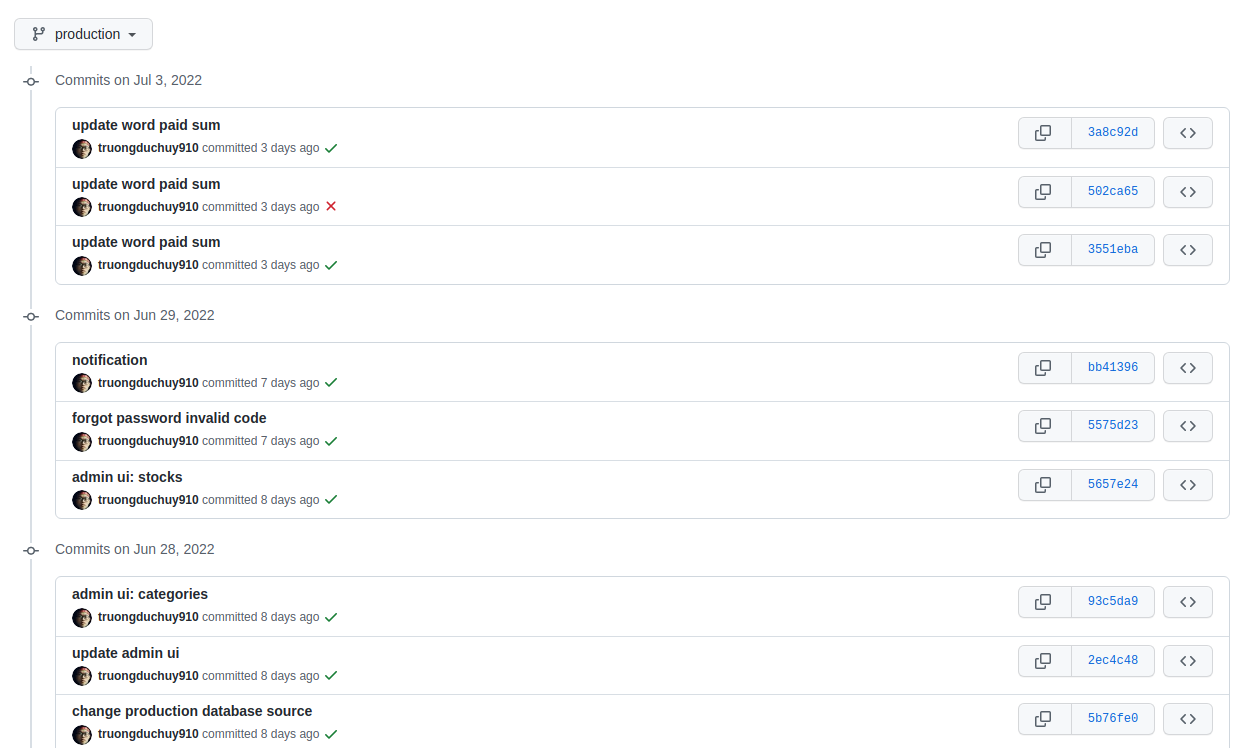
\includegraphics[width=\textwidth]{./results/commit}
		\caption{Lịch sử các phiên bản phát hành môi trường \gls{production}.}
\justifying
Các commit được triển khai thành công sẽ hiện dấu tích xanh. Khi có sự cố có thể quay về bản triển khai thành công trước đó. Là một phương án tốt khi có lỗ hổng trên môi trường \gls{production}.
	
\end{figure}
\clearpage
\FloatBarrier
\begin{figure}[!htbp]\fontsize{13px}{13px}\selectfont
\centering
		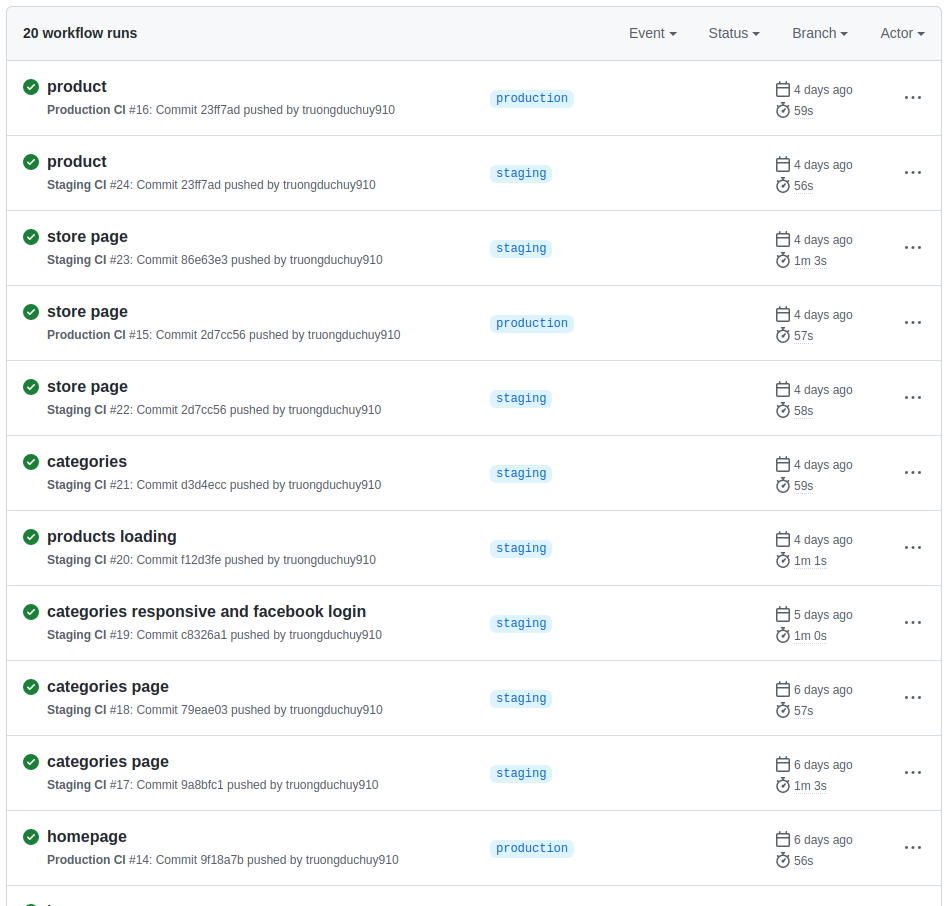
\includegraphics[width=\textwidth]{./results/deployments}
		\caption{Lịch sử cài đặt tiến trình ở các môi trường \gls{staging} và \gls{production} sử dụng CI/CD của github actions.}
\justifying
Lịch sử triển khai các commit trên các môi trường. Sau khi triển khai các tính năng trên môi trường \gls{staging} và trải qua công việc kiểm thử. Nếu không phát sinh vấn đề. Tất cả tính năng mới của \gls{staging} so với \gls{production} sẽ được triển khai bằng cách gộp mã nguồn của nhánh \gls{staging} vào nhánh \gls{production}.
	
\end{figure}
\clearpage
\begin{figure}[h!]\fontsize{13px}{13px}\selectfont
\centering
		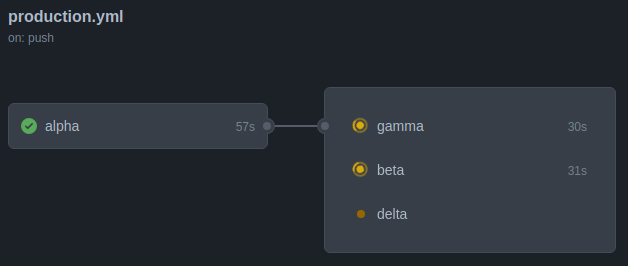
\includegraphics[width=\textwidth]{./results/jobs}
		\caption{Thông tin chi tiết khi sử dụng CI/CD chạy các bản sao của micro service trên nhiều máy chủ khác nhau}
\justifying
Hình trên mô tả máy chủ alpha là một máy chủ dự phòng của các máy chủ còn lại. Máy chủ alpha có khả năng dự phòng cho hầu hết các máy chủ dịch vụ khác. Nhưng ít khi được sử dụng. Khi việc triển diễn ra thành công trên máy chủ dự phòng, các máy chủ dịch vụ khác mới được triển khai để tránh trường hợp ảnh hưởng đến trải nghiệm phía người dùng.
\end{figure}


\begin{figure}[h!]\fontsize{13px}{13px}\selectfont
	\begin{center}	
		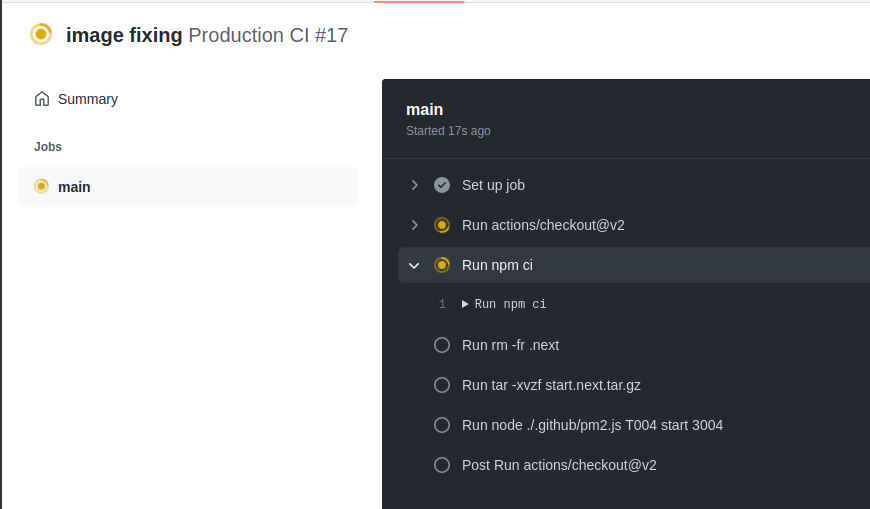
\includegraphics[width=\textwidth]{./results/production}
		\caption{Thông tin chi tiết các bước của một mirco-service sử dụng CI/CD}
	\end{center}
\end{figure}



	\fontsize{13px}{13px}\selectfont\justifying

\subsection{Kết quả}
\subsubsection{Môi trường \Gls{staging}}
\FloatBarrier
\begin{figure}[!htbp]\fontsize{13px}{13px}\selectfont
\centering
		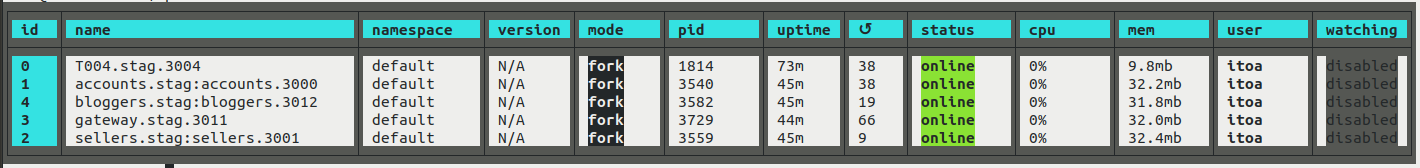
\includegraphics[width=\textwidth]{./results/vps-staging}
		\caption{Thông tin các tiến trình máy chủ \gls{staging}}
\justifying
Xem kết quả ứng dụng web tại fashion.ocopee.com
\end{figure}
\subsubsection{Môi trường \Gls{production}}
\FloatBarrier
\begin{figure}[!htbp]\fontsize{13px}{13px}\selectfont
\centering
		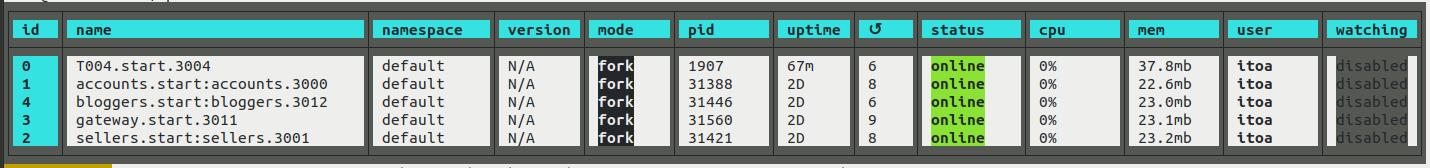
\includegraphics[width=\textwidth]{./results/vps-production}
		\caption{Thông tin các tiến trình máy chủ \gls{production}}
\justifying
Xem kết quả ứng dụng web tại ocopee.com
\end{figure}
\FloatBarrier
\begin{figure}[!htbp]\fontsize{13px}{13px}\selectfont
\centering
		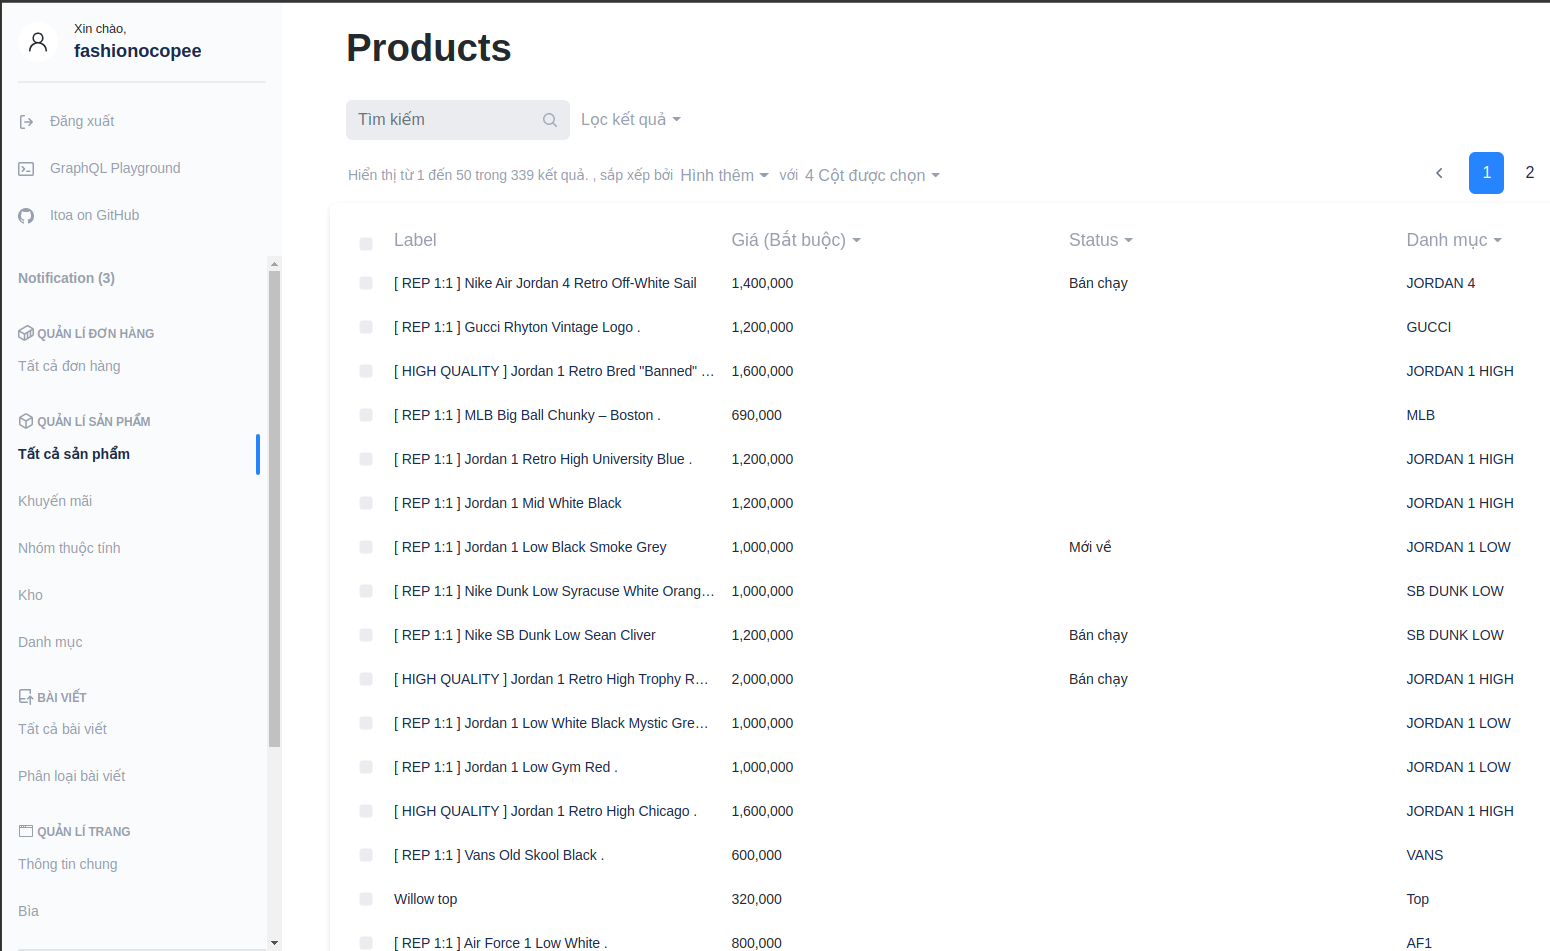
\includegraphics[width=\textwidth]{./results/product}
		\caption{Trang quản lí sản phẩm}
\justifying
\end{figure}
\clearpage
\subsubsection{Trang quản lí đơn hàng}
\FloatBarrier
\begin{figure}[!htbp]\fontsize{13px}{13px}\selectfont
\centering
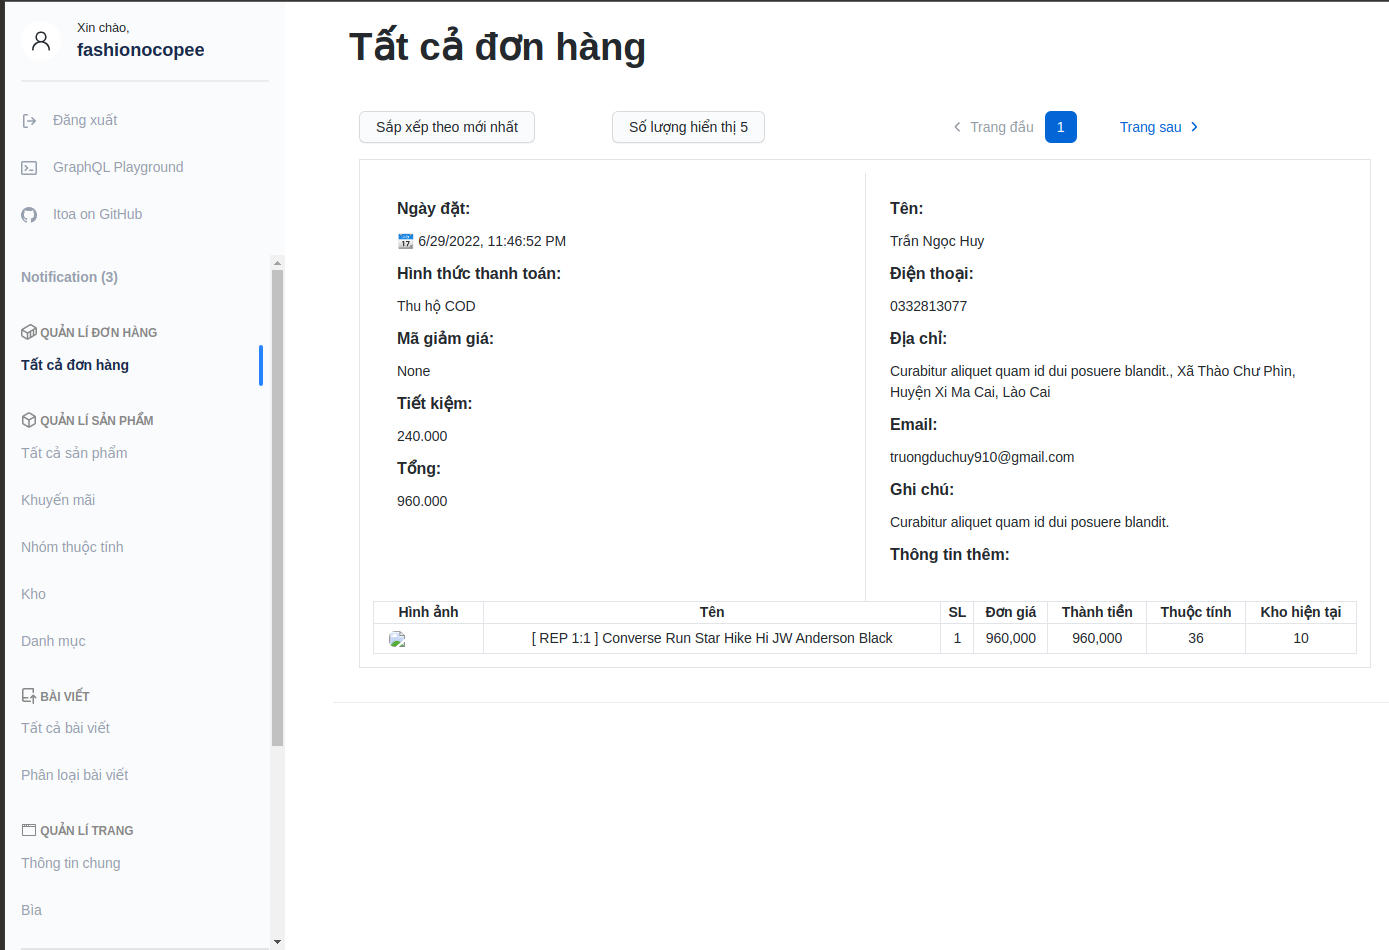
\includegraphics[width=\textwidth]{./results/order}
\caption{Trang quản lí đơn hàng}
\justifying
Trang quản lí thông tin đơn hàng dành cho nhà bán hàng cho phép nhà bán hàng xem thông tin người mua hàng để lại bao gồm: Địa chỉ nhận hàng, thông tin liên hệ, hình thức thanh toán, chi tiết đơn hàng và mã giảm giá đã sử dụng.
\end{figure}
\clearpage
\subsubsection{Trang kết bạn và chia sẻ sản phẩm}
\FloatBarrier
\begin{figure}[!htbp]\fontsize{13px}{13px}\selectfont
\centering
		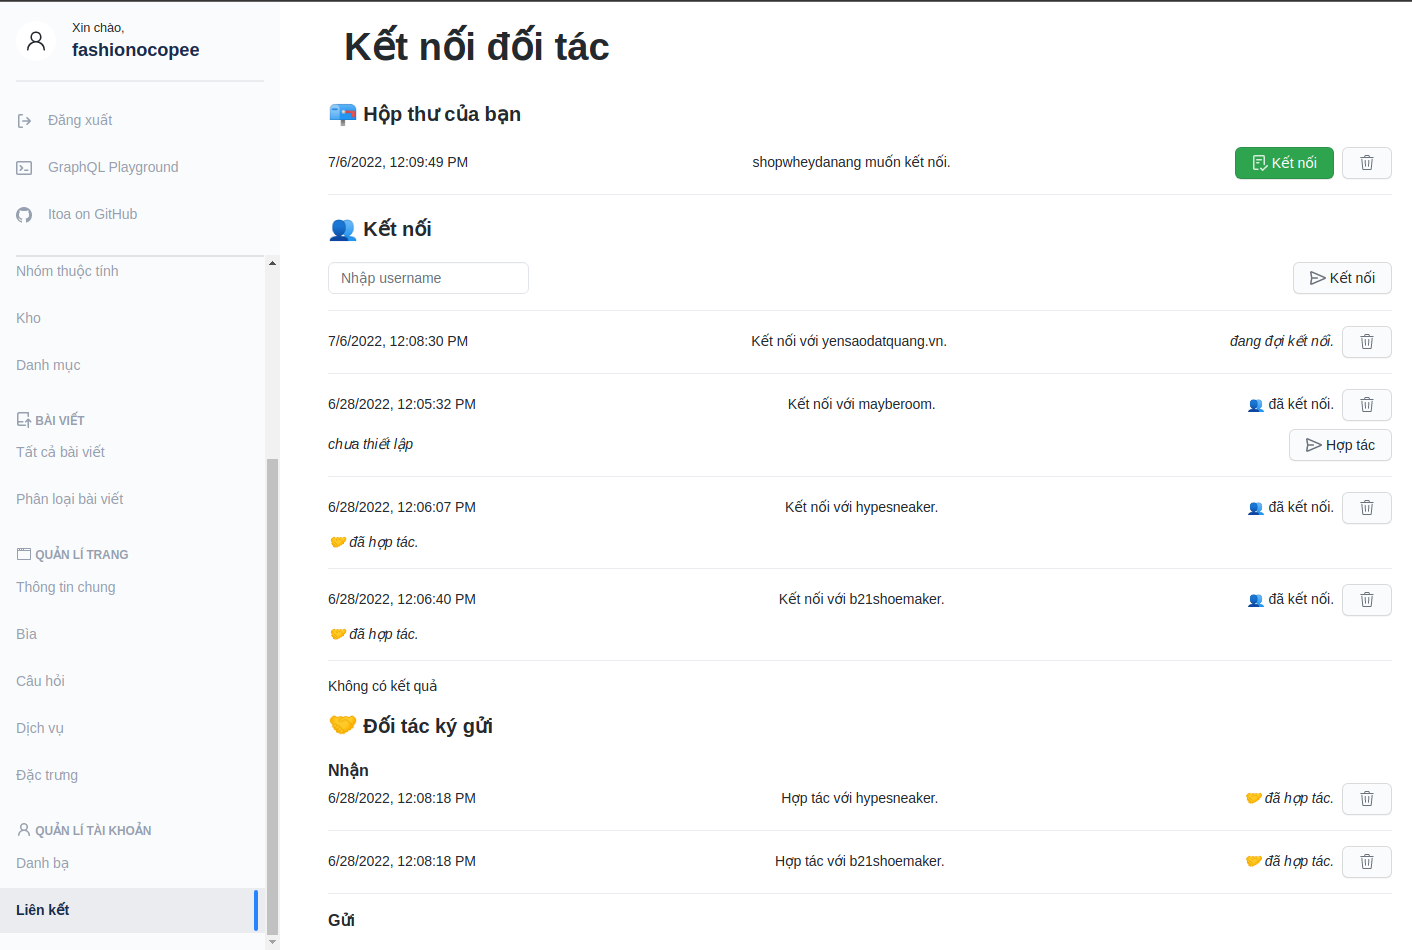
\includegraphics[width=\textwidth]{./results/contract}
		\caption{Trang kết bạn và chia sẻ sản phẩm}
\justifying
Tính năng kết bạn và chia sẻ sản phẩm được trình bày dưới dạng kết nối và ký gửi, theo cách gọi thông thường của nhà sản xuất và cửa hàng. Trước khi gửi hoặc nhận dữ liệu từ đối tác. Hai bên cần gửi lời mời kết bạn cho nhau và không quan trong người nào gửi cho người nào.

Riêng với tính năng hợp tác, người tạo yêu cầu chia sẻ sản phẩm. Tức là người bấm vào nút hợp tác trên một dòng trong danh sách đã kết nối. Người yêu cầu là người được quyền xem và trình bày thông tin sản phẩm của đối tác lên trang của mình.

Đồng nghĩa với việc, nếu nhà sản xuất chấp nhận lời mời, sản phẩm của họ sẽ được hiển thị và đăng bán trên trang của người tạo ra lời mời hợp tác.
\end{figure}
\clearpage
\subsubsection{Trang thông báo}
\FloatBarrier
\begin{figure}[!htbp]\fontsize{13px}{13px}\selectfont
\centering
		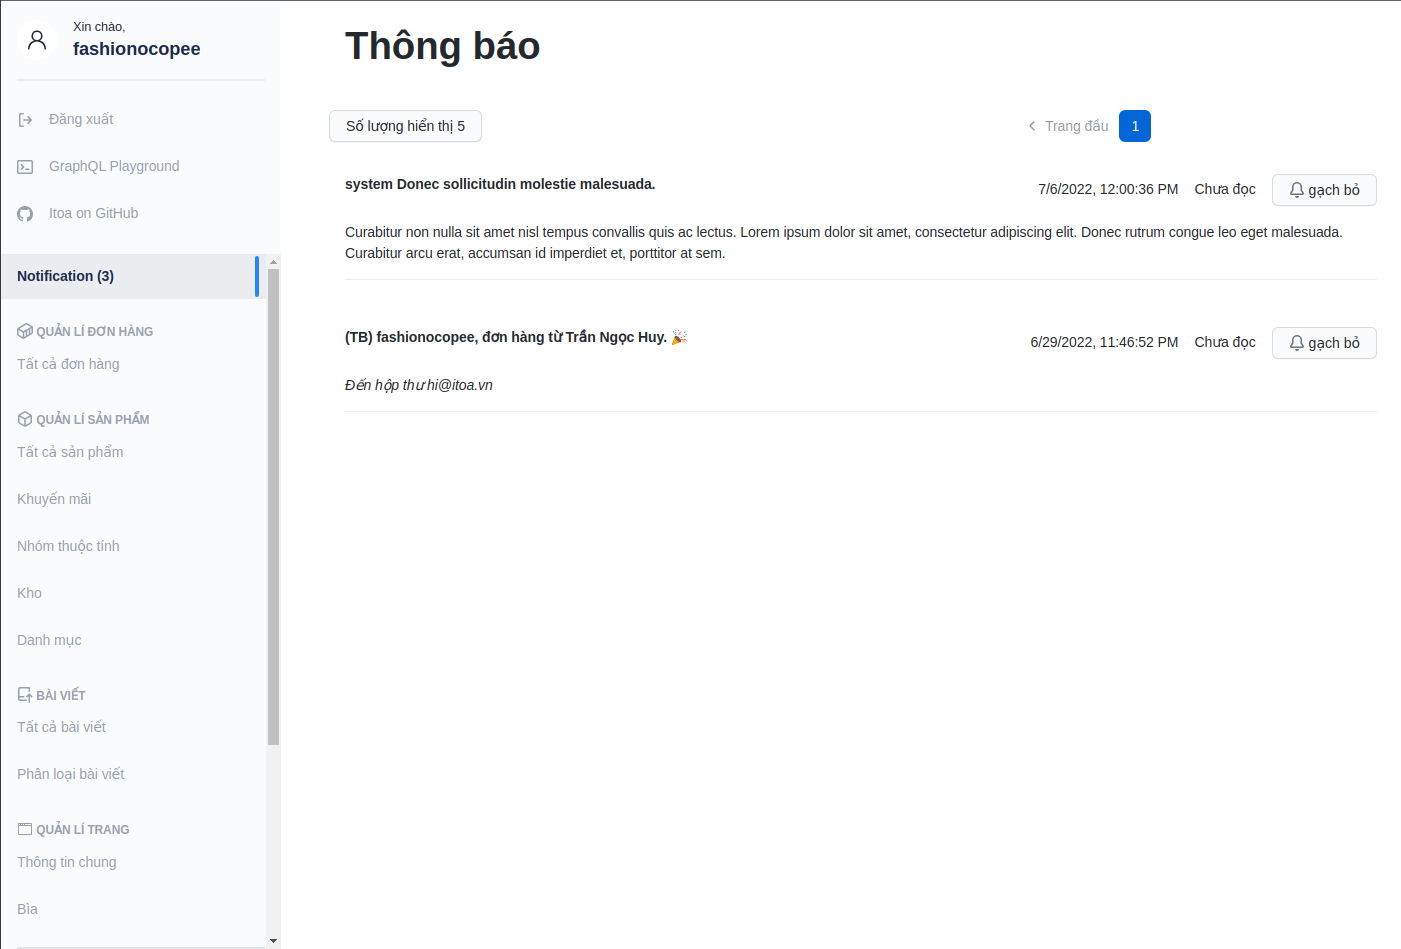
\includegraphics[width=\textwidth]{./results/notifications}
		\caption{Trang thông báo}
\justifying
Trang thông báo giúp cho nhà bán hàng hoặc nhà sản xuất kiểm tra hộp thư thông báo của mình. Đánh dấu các thông báo đã xem. Trang thông báo mặc định hiển thị ưu tiên các thông báo mới nhất chưa được xem.

Các thông báo đến địa chỉ thư điện tử của nhà bán hàng sẽ không được hiển thị nội dung mà thay vào đó. Thông báo chỉ hiển thị thông tin tiêu đề và ghi chú kiểm tra hộp thư.
\end{figure}
\clearpage
\subsubsection{Trang quản lí danh mục}
\FloatBarrier
\begin{figure}[!htbp]\fontsize{13px}{13px}\selectfont
\centering
		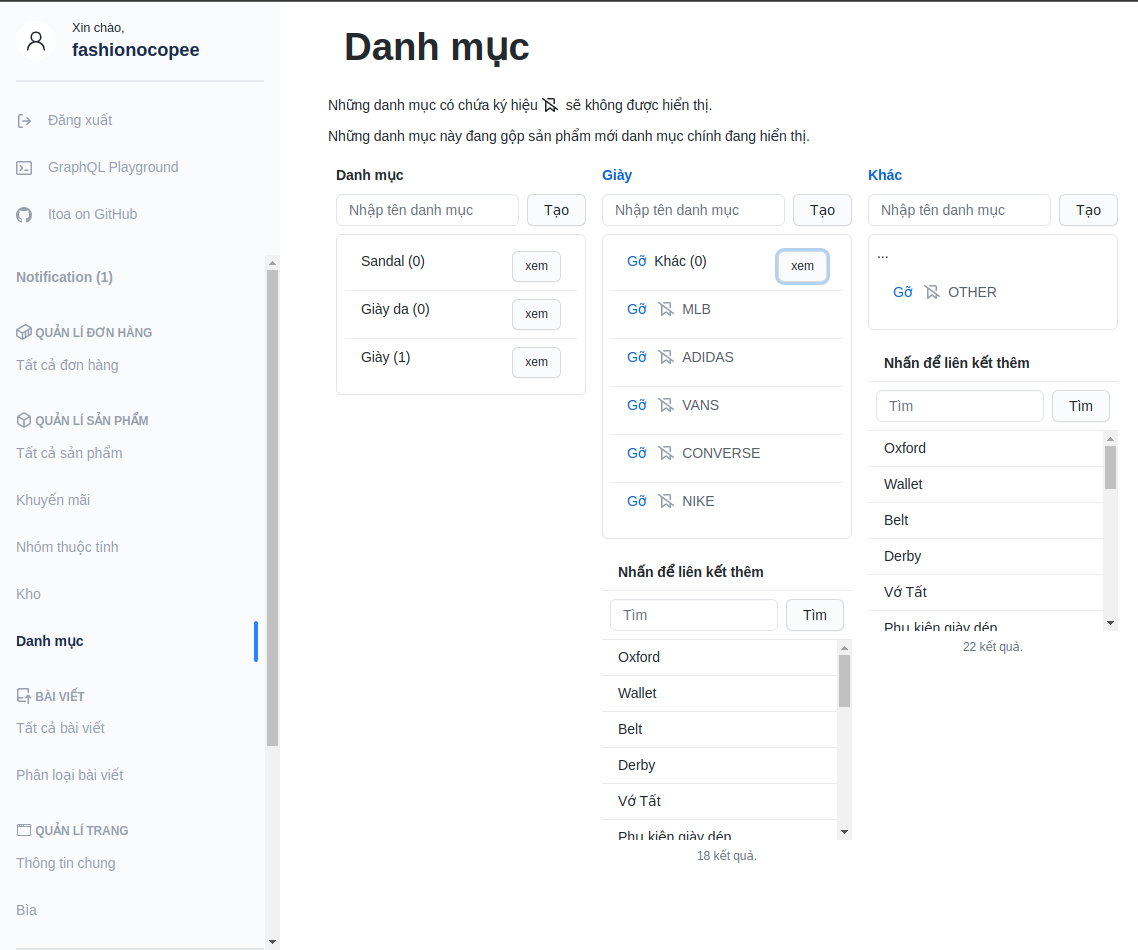
\includegraphics[width=\textwidth]{./results/categories}
		\caption{Trang quản lí danh mục}
\justifying
Quản lý danh mục giúp phân loại sản phẩm cho nhà sản xuất. Khi chia sẻ cho các nhà bán hàng. Danh mục sản phẩm có chức năng đánh dấu danh mục tương đương.

Nghĩa là đối với một nhà sản xuất hoặc nhà bán hàng. Họ luôn có cho mình cây danh mục do họ sở hữu. Và cũng là cây danh mục hiển thị chính trên trang.

Nhưng khi được chia sẻ sản phẩm, các sản phẩm được chia sẻ được liên kết với danh mục của nhà sản xuất. Và các danh mục ngoài nằm ngoài quyền quản lí của nhà bán hàng. Do vậy, tính năng danh mục tương đương đánh dấu các danh mục nào của nhà sản xuất là tương đương với danh mục của nhà bán hàng hiện tại. Sau khi đánh dấu tương được thì sản phẩm của nhà sản xuất, mặc dù nằm ngoài quyền quản lí của nhà bán hàng nhưng cũng có thể sắp xếp tìm kiếm bởi danh mục riêng của nhà bán hàng.
\end{figure}
\clearpage
\subsubsection{Trang quản lí tồn kho}
\FloatBarrier
\begin{figure}[!htbp]\fontsize{13px}{13px}\selectfont
	\centering
		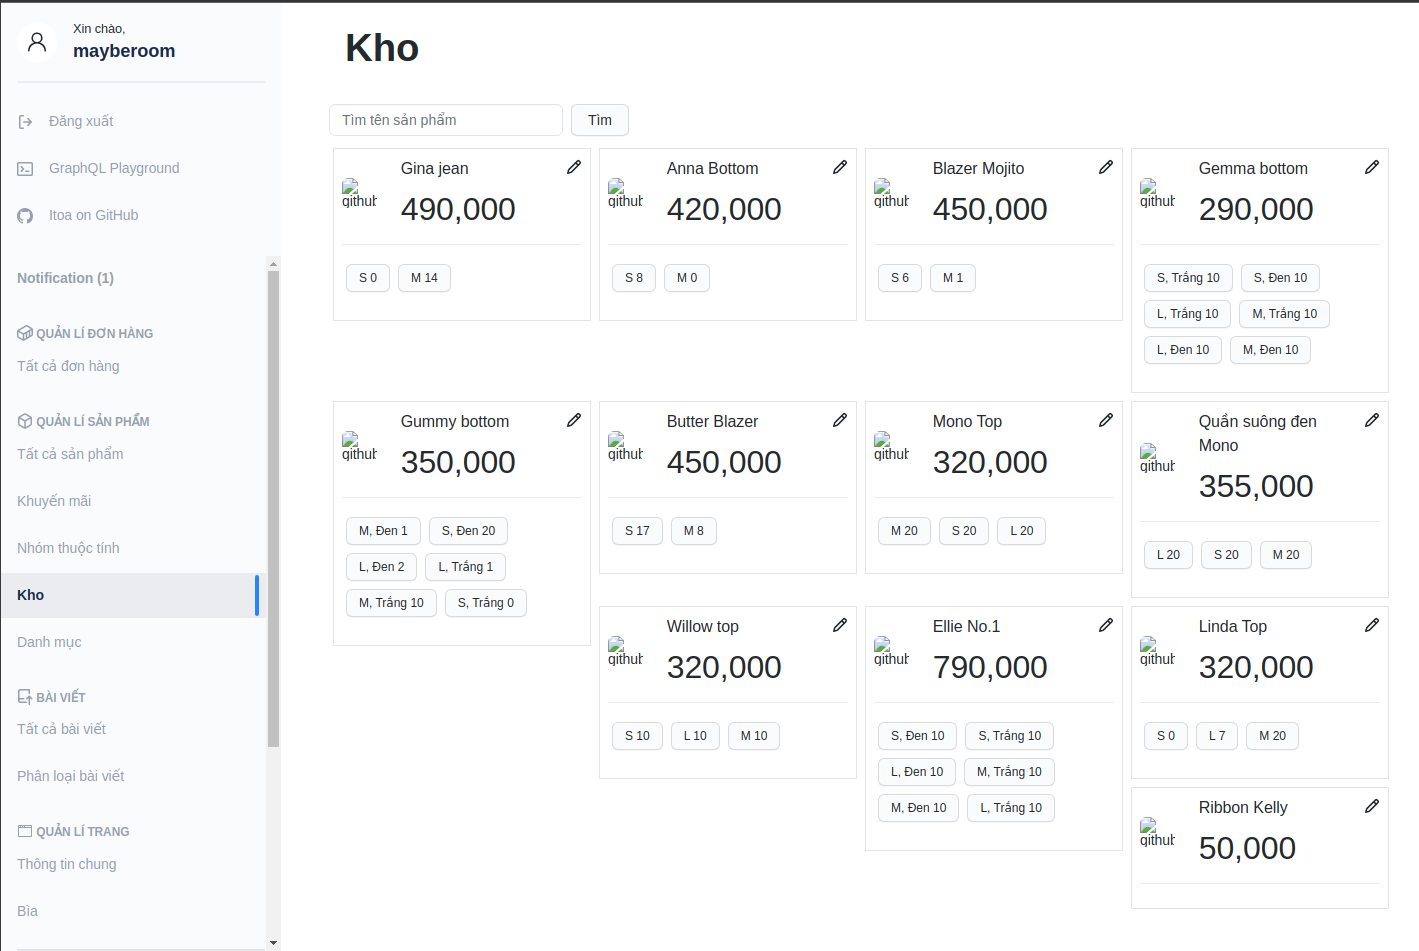
\includegraphics[width=\textwidth]{./results/stock}
		\caption{Trang quản lí tồn kho}
	\justifying
Quản lí có chức năng hiển thị tồn kho khi khách hàng chọn thuộc tính của sản phẩm. Ngăn chặn người dùng thêm nhiều hơn số tồn kho vào giỏ hàng hoặc mua sản phẩm hết hàng. Quản lí kho không bao gồm các chức năng tự động giảm số lượng trong kho khi đơn hàng sử lý thành công.
\end{figure}
\clearpage
\subsubsection{Trang quản lí thuộc tính}
\FloatBarrier
\begin{figure}[!htbp]\fontsize{13px}{13px}\selectfont
\centering
		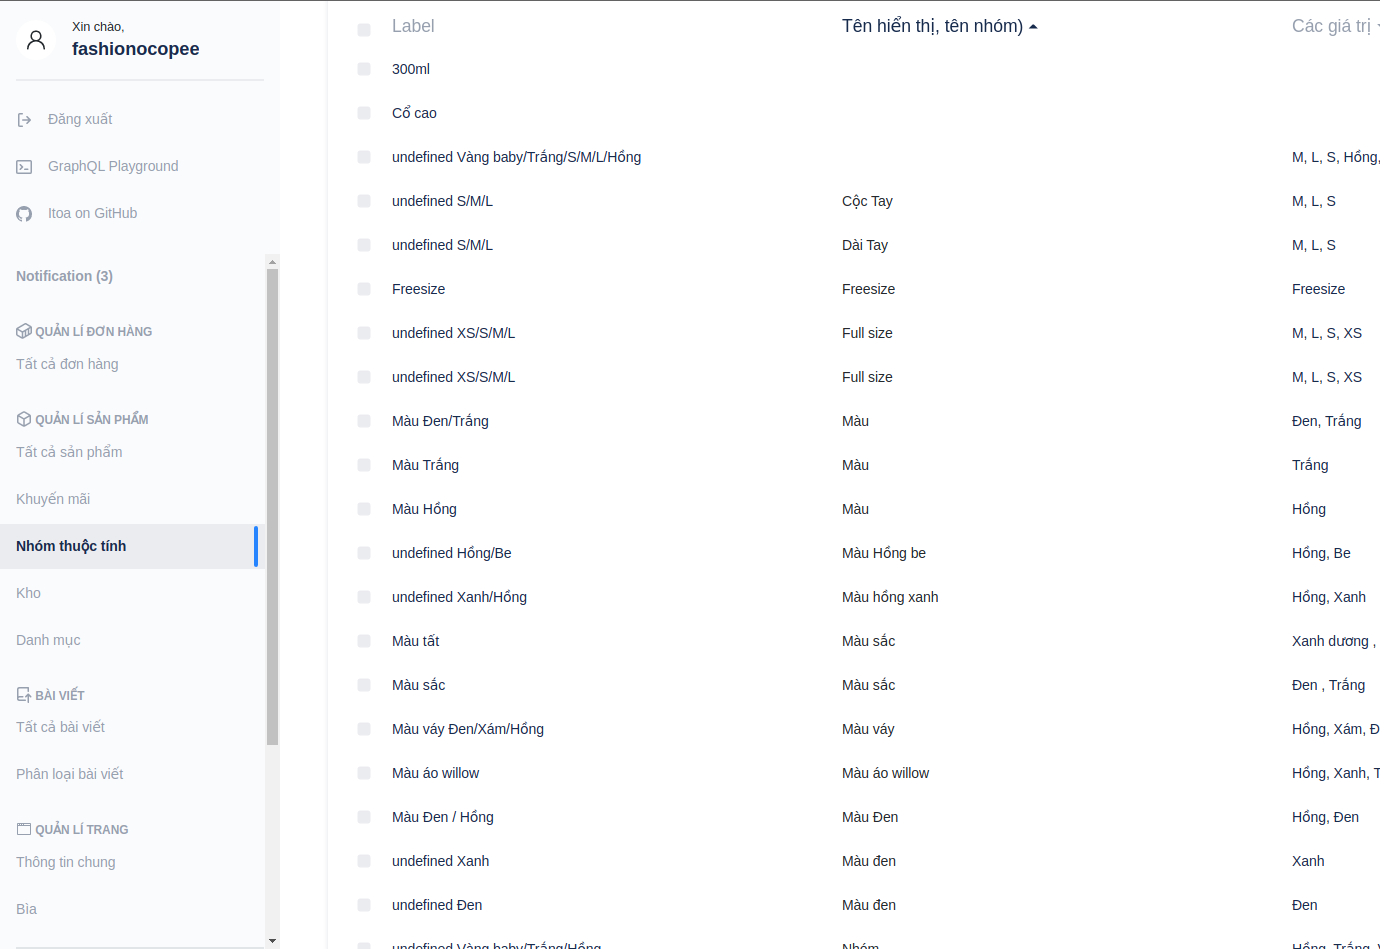
\includegraphics[width=\textwidth]{./results/attributes}
		\caption{Trang quản lí thuộc tính}
\justifying
Thuộc tính của một sản phẩm được định nghĩa là các phiên bản khác nhau của sản phẩm đó. Cùng một quy trình sản xuất hoặc cùng giá bán và chi phí sản xuất có thể cho là cùng một sản phẩm. Các thuộc tính của sản phẩm cũng được nhóm, quản lý kho và hình ảnh của thuộc tính đó. Ví dụ: kích thước, màu sắc. Cùng một sản phẩm giày nhưng khác màu sắc thì hình ảnh hiển thị cũng cần được lưu trữ và hiển thị trên trang.
\end{figure}
\clearpage
\subsubsection{Trang quản lí thông tin cửa hàng}
\FloatBarrier
\begin{figure}[!htbp]\fontsize{13px}{13px}\selectfont
\centering
		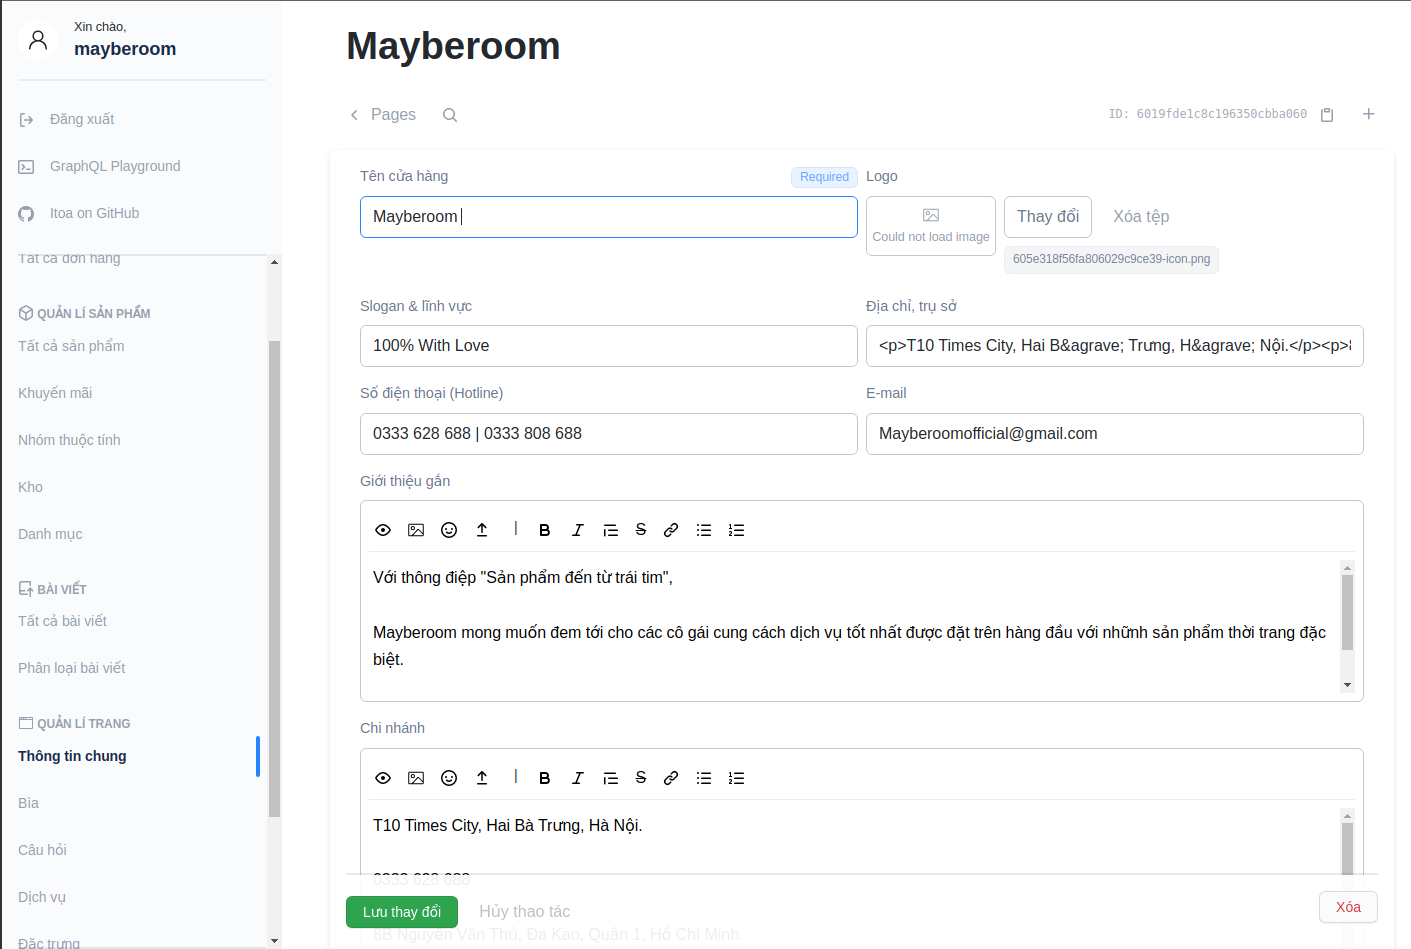
\includegraphics[width=\textwidth]{./results/store}
		\caption{Trang quản lí thông tin cửa hàng}
\justifying
Trang quản lý cửa hàng bao gồm các thông tin liên hệ cơ bản của nhà bán hàng. Các chính sách như thanh toán và vận chuyển.

Quản lí cửa hàng cũng bao gồm các thông tin thiết kế, tùy biến cá nhân hóa cho từng nhà bán hàng. Ví dụ như: Màu chủ đạo, lời chào,...
\end{figure}
\clearpage
\subsubsection{Trang quản lí mã giảm giá}
\FloatBarrier
\begin{figure}[!htbp]\fontsize{13px}{13px}\selectfont
\centering
		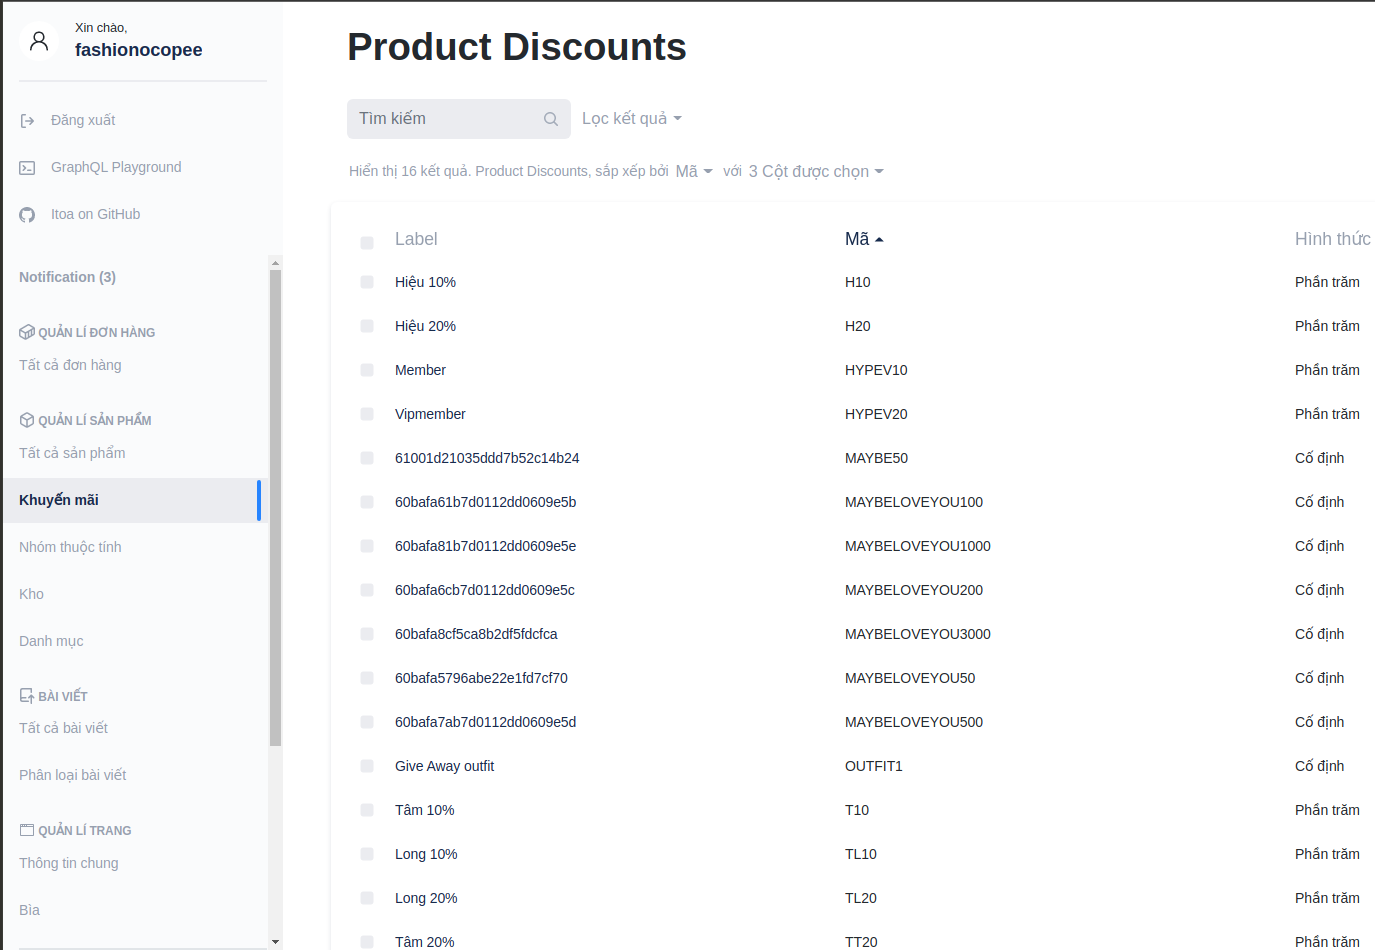
\includegraphics[width=\textwidth]{./results/discount}
		\caption{Trang quản lí mã giảm giá}
\justifying
	Trang quản lí mã khuyến mãi giúp người quản trị xem, sửa, xóa các mã khuyến mãi dựa theo phần trăm giảm. Hoặc theo giá cố định. Mã khuyến mãi cũng có thể đặt điều kiện tối thiểu để áp dụng mã giảm giá.
	
	Mã giảm giá của nhà sản xuất có thể được chia sẻ cho nhà bán hàng nhưng không thể sử dụng bởi một nhà sản xuất khác cũng cùng cung cấp sản phẩm cho nhà bán hàng.

	Mặc định mã giảm giá không thể truy cập bởi khách hàng, thông qua phiếu đặt hàng, mã giảm giá được nhập vào và kiểm tra trên hệ thống máy chủ.
\end{figure}
\clearpage
\subsubsection{Trang chủ sàn thương mại điện tử}
\FloatBarrier
\begin{figure}[!htbp]\fontsize{13px}{13px}\selectfont
\centering
		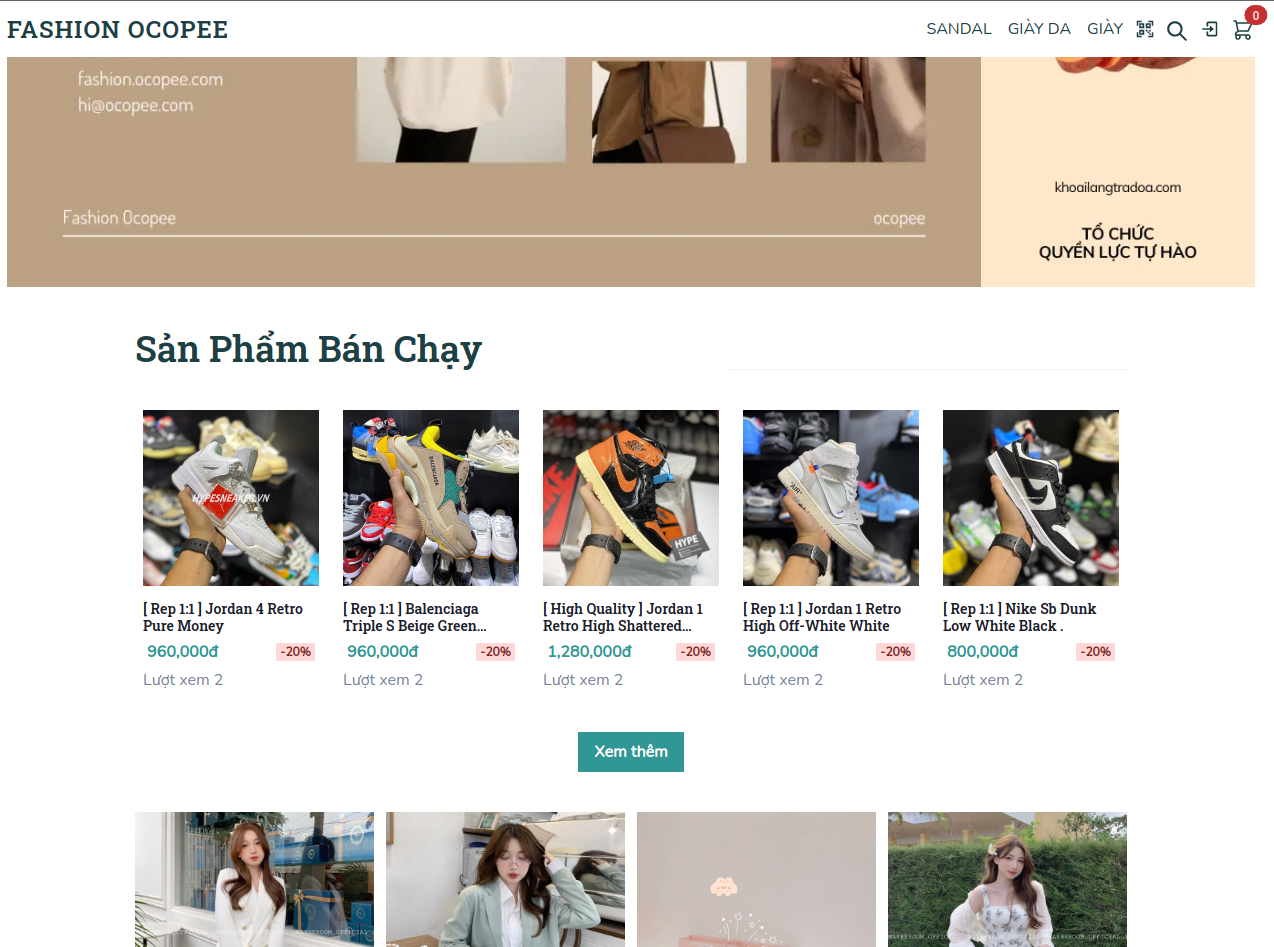
\includegraphics[width=\textwidth]{./results/homepage}
		\caption{Trang chủ sàn thương mại điện tử}
\justifying
Trang chủ sàn thương mại điện tử cho nhà bán hàng hiển thị các thông tin sản phẩm được chia sẻ cho sàn. Các hình ảnh quảng cáo. Điều hướng đến trang danh mục và chi tiết sản phẩm.
\end{figure}
\clearpage
\FloatBarrier
\begin{figure}[!htbp]\fontsize{13px}{13px}\selectfont
\centering
		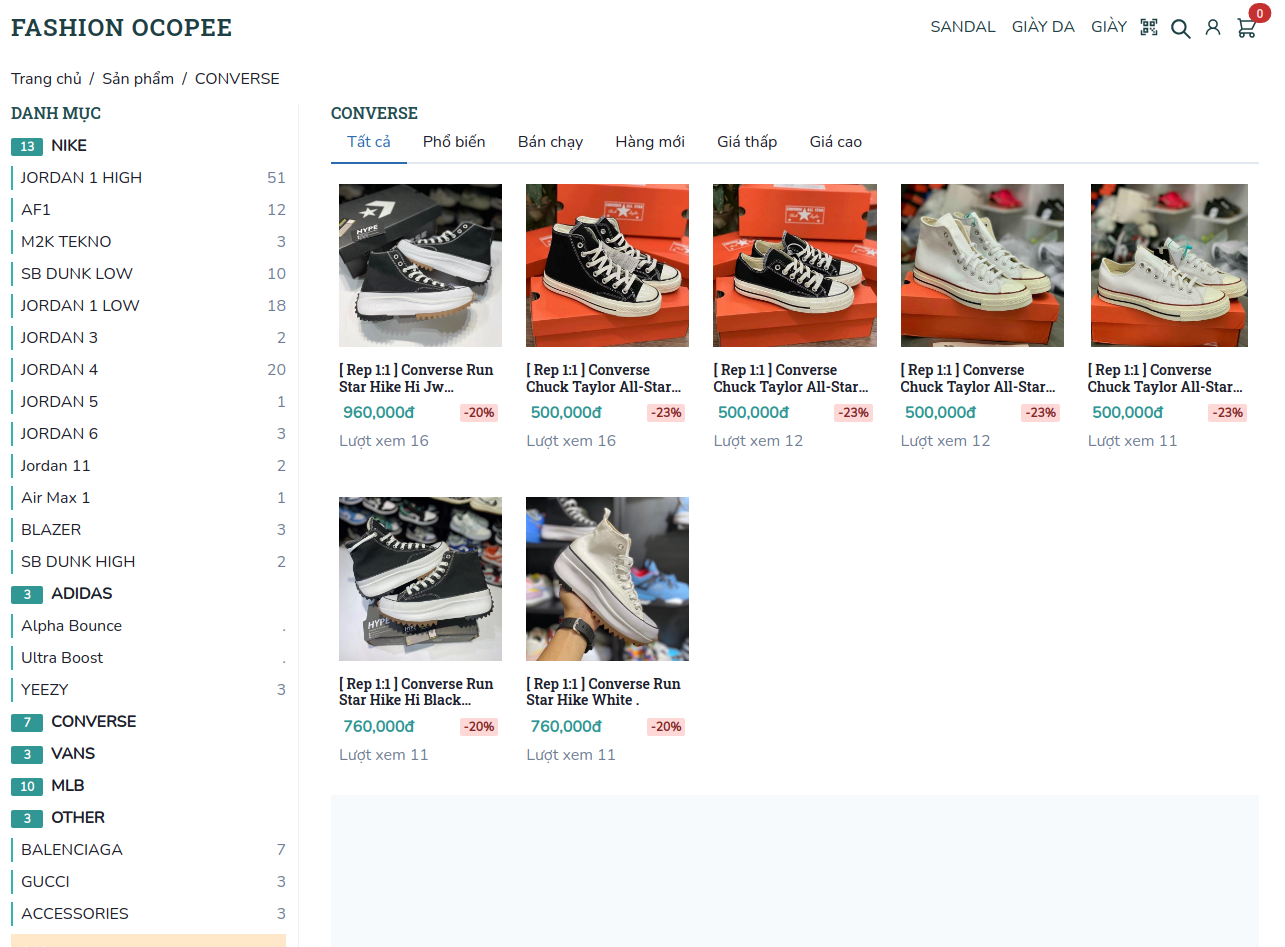
\includegraphics[width=\textwidth]{./results/categories-page}
		\caption{Trang duyệt xem sản phẩm}
\justifying
Trang duyệt xem hay còn gọi là trang trình bày sản phẩm, danh mục sản phẩm chung được quản lí bởi nhà bán hàng. Người dùng có thể xem sản phẩm theo danh mục, với các trạng thái như: bán chạy, phổ biến, hàng mới, giá thấp, giá cao... Nút xem thêm sản phẩm được thiết kế theo kiểu nối thêm sản phẩm thay vì lật trang.

\end{figure}
\clearpage
\FloatBarrier
\begin{figure}[!htbp]\fontsize{13px}{13px}\selectfont
\centering
		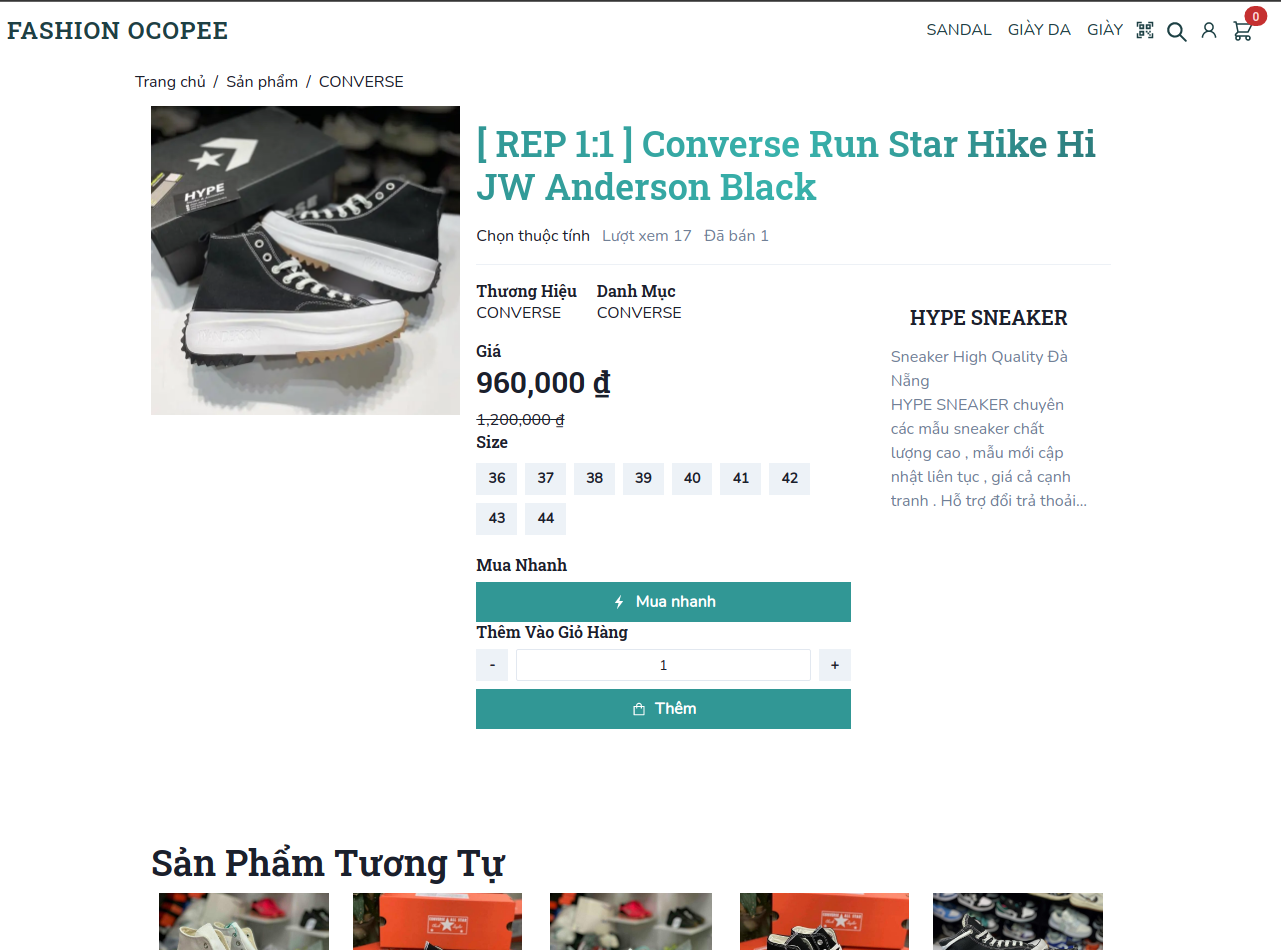
\includegraphics[width=\textwidth]{./results/product-page}
		\caption{Trang chi tiết sản phẩm}
\justifying
Trang chi tiết sản phẩm cho phép người mua hàng lựa chọn các thuộc tính của sản phẩm. Xem tồn kho của thuộc tính đó. Chức năng mua nhanh cho một sản phẩm duy nhất vào giỏ hàng và điều hướng đến trang thông tin đặt hàng. Chức năng thêm sẽ thêm số lượng sản phẩm tương ứng vào giỏ hàng. Bên cạnh thông tin chi tiết có hiển thị thông tin nhà cung cấp hoặc nhà sản xuất. Người dùng có thể đi đến không gian riêng của từng nhà sản xuất, trong trang chung hiện tại.
\end{figure}
\clearpage
\FloatBarrier
\begin{figure}[!htbp]\fontsize{13px}{13px}\selectfont
\centering
		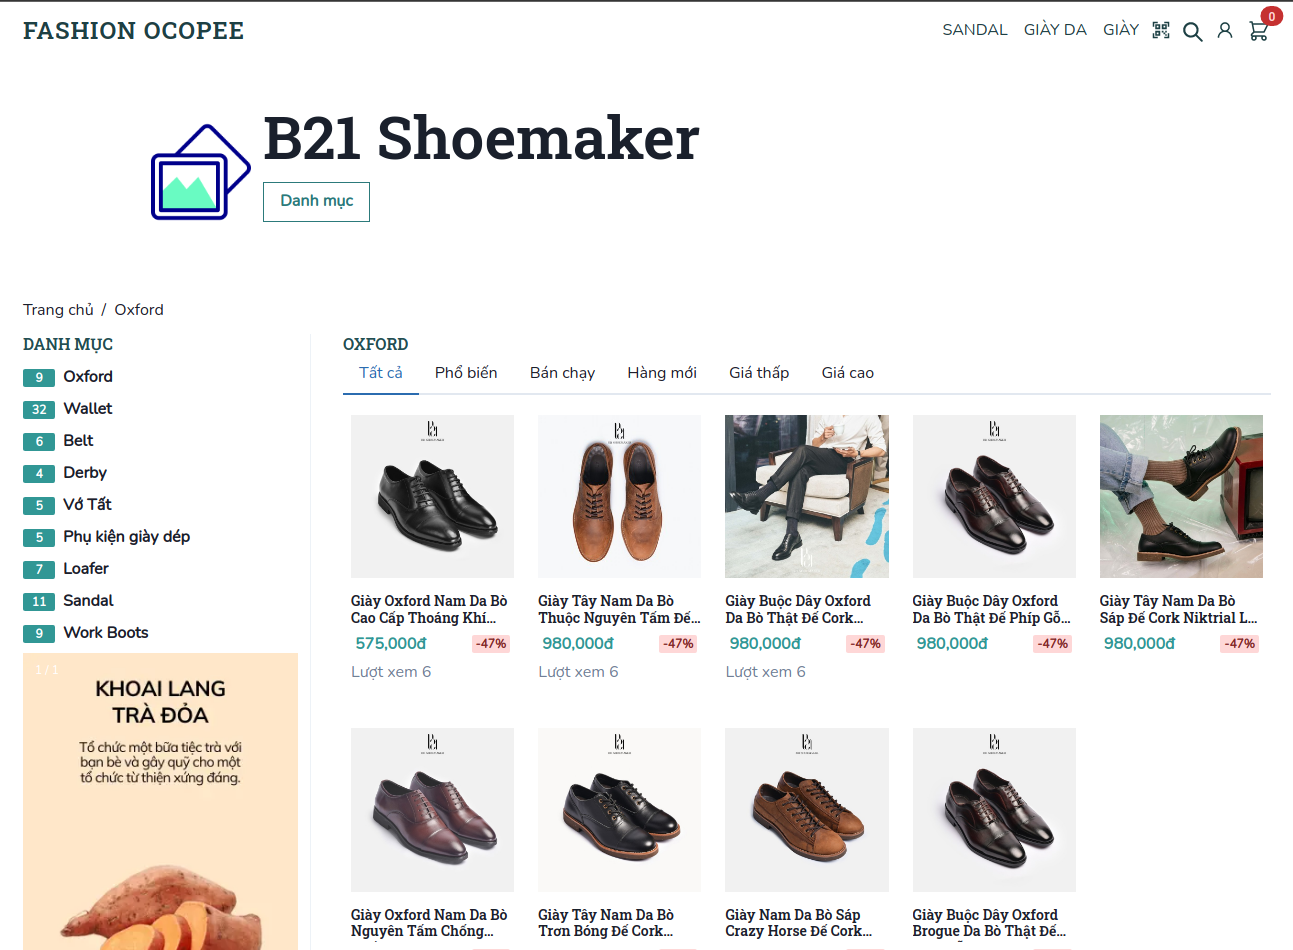
\includegraphics[width=\textwidth]{./results/store-page}
		\caption{Trang riêng của từng nhà sản xuất trên sàn}
\justifying
	Từng nhà sản xuất khi tham gia chia sẻ sản phẩm lên trang chung của nhà bán hàng cũng được xây dựng một không gian gian hàng riêng.
	Khác với trình bày sản phẩm chung, trang trình bày sản phẩm riêng cho từng nhà cung cấp, nhà sản xuất sử dụng danh mục sản phẩm được tạo ra bởi chính nhà sản xuất đó.
\end{figure}
	\fontsize{13px}{13px}\selectfont\justifying

	\section{Đánh giá}

Đồ án cơ bản đã đạt được các yêu cầu đặt ra để giải quyết vấn đề. Với các yêu cầu nêu trong phần đặc tả, sau đây là bảng đánh giá chi tiết:

	\begin{table}[h!]
	\begin{center}
		\caption{Bảng đánh giá kết quả}
		\begin{tabularx}{0.8\textwidth}{ |l|l|X| } 
			\hline
			Tên yêu cầu & Mức độ hoàn thiện & Mô tả\\
			\hline
			Yêu cầu tính năng & 90\% & Các tính năng, nghiệp vụ cơ bản được hoàn thành\\
			Yêu cầu giao diện & 85\% & Giao diện được thiết kế hiện đại, kiểm tra kỹ, chạy tốt trên các loại màn hình khác nhau. \\
			Yêu cầu hiệu suất & 75\% & Hệ thống còn một số chỗ chưa tối ưu truy vấn \\
			Yêu cầu thiết kế & 90\% & Hệ thống cơ bản đạt yêu cầu thiết kế \\
			Yêu cầu phi tính năng & 70\% & Hệ thống vẫn cần sao lưu dự phòng bằng phương pháp thủ công \\
			\hline
		\end{tabularx}

	\end{center}
\end{table}

	
	\fontsize{13px}{13px}\selectfont\justifying

\chapter*{KẾT LUẬN VÀ HƯỚNG PHÁT TRIỂN}
	% size 14
	\addcontentsline{toc}{chapter}{Kết luận}
	%	Nội dung kết luận {Font: Time New Roman; thường; cỡ chữ: 13; dãn dòng: 1,3;căn lề: justified}
	Đồ án đã vận dụng được các kiến thức nền tảng và ứng dụng các công cụ mới để phát triển hệ thống. Sau quá trình triển khai, em nhận thấy đồ án còn hạn chế ở khả năng tăng quy mô máy chủ để phục vụ cho lượng người dùng lớn. Đồng thời cũng chưa kiểm thử được hiệu suất của truy vấn dữ liệu khi lượng người dùng trở nên nhiều hơn.
	
	Đồ án sẽ tiếp tục phát triển và phục vụ thực tế cho các doanh nghiệp sản xuất. Mở rộng thêm các tính năng phù hợp với nhu cầu doanh nghiệp. Đồng thời, các tính năng quan trọng cần được mở rộng phát triển trên nhiều nền tảng hệ điều hành.
	
	\subsection*{Những vấn đề hạn chế}
	Sau khi thực hiện đồ án em nhận thấy những vấn đề hạn chế sau:
	\textbf{kiến trúc hướng dịch vụ} Kiến trúc này chỉ phù hợp cho các đồ án lớn, nhiều nhóm làm việc với nhau. Chia thành dịch vụ giúp các nhóm hoạt động độc lập với nhau. Các \gls{backlog} được chia ra hoàn thành rồi quy nạp lại để khởi chạy toàn bộ hệ thống. Song song với việc phát hành phiên các mới của các dịch vụ, việc duy trì các phiên bản ổn định cũ của dịch vụ đó cũng khá tốn kém. Thường thì các hệ thống lớn duy trì hơn 10 phiên bản.
	
	Việc sử dụng kiến trúc hướng dịch vụ cho đồ án nhỏ sẽ đẩy mức độ phức tạp lên quá mức cần thiết do phát chia cho hệ thống và cài đặt môi trường phát hành.
	
	\textbf{kết xuất giao diện phía máy khách} Việc giao tiếp thông qua \acrshort{api} và kết xuất ứng dụng phía máy khách giúp cho ứng dụng chạy mượt hơn. Nhưng đồng thời cũng làm tăng sự phụ thuộc vào lớp giao tiếp giữa máy chủ và máy khách.  \acrshort{csr}  không tối ưu đối với các máy chủ tìm kiếm hiện tại.
	
	Thay vì mô hình thông thường toàn bộ trang được kết xuất và trả về một lần cho người dùng,  \acrshort{csr}  làm cho ứng dụng phân mảnh và cần nạp tải kết xuất nhiều lần mới dẫn đến kết quả cuối cùng.
	
	\textbf{máy tìm kiếm} đồ án vẫn chưa sử dụng máy tìm kiếm để tối ưu công việc tìm kiếm.
	
	\textbf{phân tích} Hệ thống đo lường lưu lượng hoạt động tại các kiến trúc hướng dịch vụ, các cầu nối chưa được phát triển đầy đủ. Điều này giúp quá trình nâng cao hiệu suất, cải thiện độ chịu tải của hệ thống trở nên khó khăn hơn.
	
	\subsection*{Hướng phát triển}
	
	\textbf{Mạng xã hội} Hiện tại hệ thống đã có tính năng kết bạn, cần phát triển thêm tính năng tương tác của mạng xã hội. Giúp không gian mua hàng trở nên sống động hơn. Cho phép khách hàng phản hồi về sản phẩm, đánh giá, trả lời bình luận. Xem các hoạt động của người khác ở thời điểm hiện tại.
	
	\textbf{phát trực tiếp} Tính năng phát trực tiếp giúp cho nhà bán hàng xuất hiện lên tất cả các trang cho chia sẻ sản phẩm. Đồng thời cũng cần cam kết và kiểm duyệt nội dung của buổi phát trực tiếp.
	
	\textbf{Phân tích hành vi} Tính năng phân tích hành vi của người mua hàng, đánh giá mức độ ưu tiên hiển thị. Tạo nhiều tính năng giúp người dùng phản hồi nhanh về sản phẩm giúp nhà sản xuất cải thiện chất lượng.
	
	% Tham khảo
	\raggedright
	\bibliographystyle{alpha}
	\bibliography{website}
	\addcontentsline{toc}{chapter}{Tài liệu tham khảo}
\end{document}
